%%%%%%%%%%%%%%%%%%%%%%%%%%%%%%%%%%%%%%%%%%%%%%%%%%%%%%%%%%%%%%%%%%%%%%%%%%%%%%%%
%  Zawartość: Główny plik szablonu pracy dyplomowej (magisterskiej/inżynierskiej). 
%  Opracował: Tomasz Kubik <tomasz.kubik@pwr.edu.pl>
%  Data: styczeń 2023
%  Wersja: 0.9
%  Wymagania: kompilator pdflatex
%%%%%%%%%%%%%%%%%%%%%%%%%%%%%%%%%%%%%%%%%%%%%%%%%%%%%%%%%%%%%%%%%%%%%%%%%%%%%%%%

\documentclass[a4paper,onecolumn,oneside,12pt,extrafontsizes]{memoir}
%  W celu przygotowania wydruku do archiwum można:
%  a) przygotować pdf, w którym dwie strony zostaną wstawione na jedną fizyczną stronę i taki dokument wydrukować dwustronnie (podejście zalecane)
%
%   Taki dokument można przygotować poprzez
%   - wydruk z Adobe Acrobat Reader z opcją "Wiele" - sekcja "Rozmiar i obsługa stron"
%   - wykorzystanie narzędzi psutils
%
%      Windows (zakładając, że w dystrybucji MiKTeX jest pakiet miktex-psutils-bin-x64-2.9):
%        "c:\Program Files\MiKTeX 2.9\miktex\bin\x64\pdf2ps.exe" bartosz_blyszcz_mgr_2024_05_09_new.pdf Dyplom.ps
%        "c:\Program Files\MiKTeX 2.9\miktex\bin\x64\psnup.exe" -2 Dyplom.ps Dyplom2.ps
%        "c:\Program Files\MiKTeX 2.9\miktex\bin\x64\ps2pdf.exe" Dyplom2.ps Dyplom2.pdf
%        Del Dyplom2.ps Dyplom.ps
%
%     Linux:
%        pdf2ps bartosz_blyszcz_mgr_2024_05_09_new.pdf - | psnup -2 | ps2pdf - Dyplom2.pdf
%
%  b) przekomplilować dokument zmniejszając czcionkę (podejście niezalecane, bo zmienia formatowanie dokumentu)
%
%    Do tego wystarczy posłużyć się poniższymi komendami (zamiast documentclass z pierwszej linijki):
%   \documentclass[a4paper,onecolumn,twoside,10pt]{memoir} 
%   \renewcommand{\normalsize}{\fontsize{8pt}{10pt}\selectfont}

%\usepackage[cp1250]{inputenc} % Proszę zostawić, jeśli kodowanie edytowanych plików to cp1250 
\usepackage[utf8]{inputenc} % Proszę użyć zamiast powyższego, jeśli kodowanie edytowanych plików to UTF8
\usepackage[T1]{fontenc}
\usepackage[english,polish]{babel} % Tutaj ważna jest kolejność atrybutów (dla pracy po polsku polish powinno być na końcu)
%\DisemulatePackage{setspace}
\usepackage{setspace}
\usepackage{color,calc}
%\usepackage{soul} % pakiet z komendami do podkreślania, przekreślania, podświetlania tekstu (raczej niepotrzebny)
\usepackage{ebgaramond} % pakiet z czcionkami garamond, potrzebny tylko do strony tytułowej, musi wystąpić przed pakietem tgtermes

%% Aby uzyskać polskie literki w pdfie (a nie zlepki) korzystamy z pakietu czcionek tgterms. 
%% W pakiecie tym są zdefiniowane klony czcionek Times o kształtach: normalny, pogrubiony, italic, italic pogrubiony.
%% W pakiecie tym brakuje czcionki o kształcie: slanted (podobny do italic). 
%% Jeśli w dokumencie gdzieś zostanie zastosowana czcionka slanted (np. po użyciu komendy \textsl{}), to
%% latex dokona podstawienia na czcionkę standardową i zgłosi to w ostrzeżeniu (warningu).
%% Ponadto tgtermes to czcionka do tekstu. Wszelkie matematyczne wzory będą sformatowane domyślną czcionką do wzorów.
%% Jeśli wzory mają być sformatowane z wykorzystaniem innych czcionek, trzeba to jawnie zadeklarować.

%% Po zainstalowaniu pakietu tgtermes może będzie trzeba zauktualizować informacje 
%% o dostępnych fontach oraz mapy. Można to zrobić z konsoli (jako administrator)
%% initexmf --admin --update-fndb
%% initexmf --admin --mkmaps

\usepackage{tgtermes}   
\renewcommand*\ttdefault{txtt}


%%%%%%%%%%%%%%%%%%%%%%%%%%%%%%%%%%%%%%%%%%%%%%%%%%%%%%%%%%%%%%%%%%%%%%%%%%%%%%%%
%% Ustawienia odpowiedzialne za sposób łamania dokumentu
%% i ułożenie elementów pływających
%%%%%%%%%%%%%%%%%%%%%%%%%%%%%%%%%%%%%%%%%%%%%%%%%%%%%%%%%%%%%%%%%%%%%%%%%%%%%%%%
%\hyphenpenalty=10000		% nie dziel wyrazów zbyt często
\clubpenalty=10000      % kara za sierotki
\widowpenalty=10000     % nie pozostawiaj wdów
%\brokenpenalty=10000		% nie dziel wyrazów między stronami - trzeba było wyłączyć, bo nie łamały się linie w lstlisting
%\exhyphenpenalty=999999		% nie dziel słów z myślnikiem - trzeba było wyłączyć, bo nie łamały się linie w lstlisting
\righthyphenmin=3			  % dziel minimum 3 litery

%\tolerance=4500
%\pretolerance=250
%\hfuzz=1.5pt
%\hbadness=1450

\renewcommand{\topfraction}{0.95}
\renewcommand{\bottomfraction}{0.95}
\renewcommand{\textfraction}{0.05}
\renewcommand{\floatpagefraction}{0.35}

%%%%%%%%%%%%%%%%%%%%%%%%%%%%%%%%%%%%%%%%%%%%%%%%%%%%%%%%%%%%%%%%%%%%%%%%%%%%%%%%
%%  Ustawienia rozmiarów: tekstu, nagłówka i stopki, marginesów
%%  dla dokumentów klasy memoir 
%%%%%%%%%%%%%%%%%%%%%%%%%%%%%%%%%%%%%%%%%%%%%%%%%%%%%%%%%%%%%%%%%%%%%%%%%%%%%%%%
\setlength{\headsep}{10pt} 
\setlength{\headheight}{13.6pt} % wartość baselineskip dla czcionki 11pt tj. \small wynosi 13.6pt
\setlength{\footskip}{\headsep+\headheight}
\setlength{\uppermargin}{\headheight+\headsep+1cm}
\setlength{\textheight}{\paperheight-\uppermargin-\footskip-1.5cm}
\setlength{\textwidth}{\paperwidth-5cm}
\setlength{\spinemargin}{2.5cm}
\setlength{\foremargin}{2.5cm}
\setlength{\marginparsep}{2mm}
\setlength{\marginparwidth}{2.3mm}
%\settrimmedsize{297mm}{210mm}{*}
%\settrims{0mm}{0mm}	
\checkandfixthelayout[fixed] % konieczne, aby się dobrze wszystko poustawiało
%%%%%%%%%%%%%%%%%%%%%%%%%%%%%%%%%%%%%%%%%%%%%%%%%%%%%%%%%%%%%%%%%%%%%%%%%%%%%%%%
%%  Ustawienia odległości linii, wcięć, odstępów
%%%%%%%%%%%%%%%%%%%%%%%%%%%%%%%%%%%%%%%%%%%%%%%%%%%%%%%%%%%%%%%%%%%%%%%%%%%%%%%%
\linespread{1}
%\linespread{1.241}
\setlength{\parindent}{14.5pt}


\usepackage{multicol} % pakiet umożliwiający stworzenie wielokolumnowego tekstu
%%%%%%%%%%%%%%%%%%%%%%%%%%%%%%%%%%%%%%%%%%%%%%%%%%%%%%%%%%%%%%%%%%%%%%%%%%%%%%%%
%% Pakiety do formatowania tabel
%%%%%%%%%%%%%%%%%%%%%%%%%%%%%%%%%%%%%%%%%%%%%%%%%%%%%%%%%%%%%%%%%%%%%%%%%%%%%%%%
\usepackage{float}
\usepackage{array}
\usepackage{tabularx}
\usepackage{multirow}
\usepackage{booktabs}
\usepackage{makecell}
\usepackage[flushleft]{threeparttable}
\usepackage{nicematrix}
\usepackage{colortbl}
\usepackage{hhline}
\usepackage{subcaption}
\usepackage{enumerate}
\usepackage{diagbox}
\usepackage{csvsimple}
\usepackage{lscape}

% defines the X column to use m (\parbox[c]) instead of p (`parbox[t]`)
\newcolumntype{C}[1]{>{\hsize=#1\hsize\centering\arraybackslash}X}
\newcolumntype{P}[1]{>{\centering\arraybackslash}p{#1}}
\newcolumntype{M}[1]{>{\centering\arraybackslash}m{#1}}
\newcolumntype{L}[1]{>{\raggedright\arraybackslash}m{#1}}
% Proszę używać tylko tabularx. Innych pakietów proszę nie stosować !!!
% Dokument na pewno da się zredagować bez ich użycia.
%\usepackage{longtable}
%\usepackage{ltxtable}
%\usepackage{tabulary}

%%%%%%%%%%%%%%%%%%%%%%%%%%%%%%%%%%%%%%%%%%%%
% Grafy
%%%%%%%%%%%%%%%%%%%%%%%%%%%%%%%%%%%%%%%%%%
\usepackage{tikz}
\usetikzlibrary{shapes.symbols}
\usetikzlibrary{shapes.geometric}
\usetikzlibrary{shapes.arrows}
\tikzstyle{startstop} = [rectangle, rounded corners, minimum width=3cm, minimum height=1cm,text centered, draw=black, fill=strongorange!50]
\tikzstyle{io} = [trapezium, trapezium left angle=70, trapezium right angle=110, minimum width=3cm, minimum height=1cm, text centered, draw=black, fill=blue!30]
\tikzstyle{process} = [rectangle, minimum width=3cm, minimum height=1cm, text centered, draw=black, fill=lighteryellow!30]
\tikzstyle{decision} = [diamond, minimum width=3cm, minimum height=1cm, text centered, draw=black, fill=lightblue!50, align=center]
\tikzstyle{arrow} = [thick,->,>=stealth]
\tikzstyle{backarrow} = [thick,<-,>=stealth]

% =============================================================================
% SEC:   Kolory
% =============================================================================

\definecolor{darkgreen}{RGB}{  0 104  56}
\definecolor{lightblue}{RGB}{181 212 239}
\definecolor{strongorange}{RGB}{247 148  30}
\definecolor{lighteryellow}{RGB}{242 245 205}
\definecolor{lightred}{RGB}{252 134 134}
\definecolor{lightgreen}{RGB}{134 252 167}

%%%%%%%%%%%%%%%%%%%%%%%%%%%%%%%%%%%%%%%%%%%%%%%%%%%%%%%%%%%%%%%%%%%%%%%%%%%%%%%%
%% Pakiet do wstawiania fragmentów kodu
%%%%%%%%%%%%%%%%%%%%%%%%%%%%%%%%%%%%%%%%%%%%%%%%%%%%%%%%%%%%%%%%%%%%%%%%%%%%%%%%
\usepackage{listings} 
\usepackage{xpatch}
\makeatletter
\xpatchcmd\l@lstlisting{1.5em}{0em}{}{}
\makeatother
% Pakiet dostarcza otoczenia lstlisting. Jest ono wysoce konfigurowalne. 
% Konfigurować można indywidualnie każdy z listingów lub globalnie, w poleceniu \lstset{}.

% Zalecane jest, by kod źródłowy był wyprowadzany z użyciem czcionki maszynowej \ttfamily
% Ponieważ kod źródłowy, nawet po obcięciu do interesujących fragmentów, bywa obszerny, należy zmniejszyć czcionkę.
% Zalecane jest \small (dla krótkich fragmentów) oraz \footnotesize (dla dłuższych fragmentów).

% Ponadto podczas konfiguracji można zadeklarować sposób numerowania linii. Numerowanie linii zalecane jest jednak 
% tylko w przypadkach, gdy w redagowanym tekście znajdują się jakieś odwołania do konkretnych linii.
% Jeśli takich odwołań nie ma, numerowanie linii jest zbędne. Proszę wtedy go nie stosować.
% Przy włączaniu numerowania linii należy zwrócić uwagę na to, gdzie pojawią się te numery.
% Bez zmiany dodatkowych parametrów pojawiają się one na marginesie strony (co jest niepożądane).

\lstset{
  basicstyle=\small\ttfamily, % lub basicstyle=\footnotesize\ttfamily
  %%columns=fullflexible,
	%%showstringspaces=false,
	%%showspaces=false,
  breaklines=true,
  postbreak=\mbox{\textcolor{red}{$\hookrightarrow$}\space}, 
  %%numbers=left,  % ta i poniższe linie dotyczą ustawienia numerowania i sposobu jego wyprowadzania
  %%firstnumber=1, 
  %%numberfirstline=true, 
	%%xleftmargin=17pt,
  %%framexleftmargin=17pt,
  %%framexrightmargin=5pt,
  %%framexbottommargin=4pt,
	belowskip=.5\baselineskip,
	literate={\_}{{\_\allowbreak}}1 % ta deklaracja przydaje się, jeśli na listingu mają być łamane nazwy zawierające podkreślniki
}

% Jeśli edytowany plik nie jest w kodowaniu cp1250, to jest problem z polskimi znakami występującymi we wstawianym kodzie.
% Dlatego podczas pracy na plikach w kodowaniu UTF8 trzeba zadeklarować mapowanie jak niżej (wystarczy odmarkować).
% Niestety, jak się zastosuje to mapowanie mogą pojawić się problemy z podświetlaniem składni (patrz dalej).
\lstset{literate=%-
{ą}{{\k{a}}}1 {ć}{{\'c}}1 {ę}{{\k{e}}}1 {ł}{{\l{}}}1 {ń}{{\'n}}1 {ó}{{\'o}}1 {ś}{{\'s}}1 {ż}{{\.z}}1 {ź}{{\'z}}1 {Ą}{{\k{A}}}1 {Ć}{{\'C}}1 {Ę}{{\k{E}}}1 {Ł}{{\L{}}}1 {Ń}{{\'N}}1 {Ó}{{\'O}}1 {Ś}{{\'S}}1 {Ż}{{\.Z}}1 {Ź}{{\'Z}}1 
    {Ö}{{\"O}}1
    {Ä}{{\"A}}1
    {Ü}{{\"U}}1
    {ß}{{\ss}}1
    {ü}{{\"u}}1
    {ä}{{\"a}}1
    {ö}{{\"o}}1
    {~}{{\textasciitilde}}1
		{—}{{{\textemdash} }}1
}%{\ \ }{{\ }}1}


%% lstlisting pozwala na ostylowania podświetlania składni wybranych języków.
%% Działa to na zasadzie zdefiniowania słów kluczowych oraz sposobu ich wyświetlania.
%% Ponieważ jest to prosty mechanizm, czasem trudno osiągnąć takie efekty, jakie dają narzędzia IDE. 
%% Jednak w większości przypadku osiągane rezutlaty są zadowalające.


%% lstlisting obsługuje domyślnie kilka najpopularniejszych języków.
%%\lstloadlanguages{% Check Dokumentation for further languages ...
%%C,
%%C++,
%%csh,
%%Java
%%}
%% Inne języki muszą być dodefiniowane. Poniżej podano przykłady definicji języków i styli.

\definecolor{lightgray}{rgb}{.9,.9,.9}
\definecolor{darkgray}{rgb}{.4,.4,.4}
\definecolor{purple}{rgb}{0.65, 0.12, 0.82}
\definecolor{javared}{rgb}{0.6,0,0} % for strings
\definecolor{javagreen}{rgb}{0.25,0.5,0.35} % comments
\definecolor{javapurple}{rgb}{0.5,0,0.35} % keywords
\definecolor{javadocblue}{rgb}{0.25,0.35,0.75} % javadoc
 
\lstdefinelanguage{JavaScript}{ 
	keywords={typeof, new, true, false, catch, function, return, null, catch, switch, var, if, in, while, do, else, case, break},
	keywordstyle=\color{blue}\bfseries,
	ndkeywords={class, export, boolean, throw, implements, import, this},
	ndkeywordstyle=\color{darkgray}\bfseries,
	identifierstyle=\color{black},
	sensitive=false,
	comment=[l]{//},
	morecomment=[s]{/*}{*/},
	commentstyle=\color{purple}\ttfamily,
	stringstyle=\color{red}\ttfamily,
	morestring=[b]',
	morestring=[b]"
}
\lstdefinestyle{JavaScriptStyle}{
	language=JavaScript,
	commentstyle=\color{javagreen}, % niestety, jeśli w linii komentarza pojawią się słowa kluczowe, to zostaną pokolorowane
	backgroundcolor=,%\color{lightgray}, % można ustwić kolor tła, ale jest to niezalecane
	extendedchars=true,
	basicstyle=\footnotesize\ttfamily,
	showstringspaces=false,
	showspaces=false,
	numbers=none,%left,
	numberstyle=\footnotesize,
	numbersep=9pt,
	tabsize=2,
	breaklines=true,
	showtabs=false,
	captionpos=t
}

\lstdefinestyle{JavaStyle}{
basicstyle=\footnotesize\ttfamily,
keywordstyle=\color{javapurple}\bfseries,
stringstyle=\color{javared},
commentstyle=\color{javagreen},
morecomment=[s][\color{javadocblue}]{/**}{*/},
numbers=none,%left,
numberstyle=\tiny\color{black},
stepnumber=2,
numbersep=10pt,
tabsize=4,
showspaces=false,
showstringspaces=false,
captionpos=t
}

\definecolor{pblue}{rgb}{0.13,0.13,1}
\definecolor{pgreen}{rgb}{0,0.5,0}
\definecolor{pred}{rgb}{0.9,0,0}
\definecolor{pgrey}{rgb}{0.46,0.45,0.48}
\definecolor{dark-grey}{rgb}{0.4,0.4,0.4}
% styl json
\newcommand\JSONnumbervaluestyle{\color{blue}}
\newcommand\JSONstringvaluestyle{\color{red}}

\newif\ifcolonfoundonthisline

\makeatletter

\lstdefinestyle{json-style}  
{
	showstringspaces    = false,
	keywords            = {false,true},
	alsoletter          = 0123456789.,
	morestring          = [s]{"}{"},
	stringstyle         = \ifcolonfoundonthisline\JSONstringvaluestyle\fi,
	MoreSelectCharTable =%
	\lst@DefSaveDef{`:}\colon@json{\processColon@json},
	basicstyle          = \footnotesize\ttfamily,
	keywordstyle        = \ttfamily\bfseries,
	numbers				= left, % zakomentować, jeśli numeracja linii jest niepotrzebna
	numberstyle={\footnotesize\ttfamily\color{dark-grey}},
	xleftmargin			= 2em % zakomentować, jeśli numeracja linii jest niepotrzebna
}

\newcommand\processColon@json{%
	\colon@json%
	\ifnum\lst@mode=\lst@Pmode%
	\global\colonfoundonthislinetrue%
	\fi
}

\lst@AddToHook{Output}{%
	\ifcolonfoundonthisline%
	\ifnum\lst@mode=\lst@Pmode%
	\def\lst@thestyle{\JSONnumbervaluestyle}%
	\fi
	\fi
	\lsthk@DetectKeywords% 
}

\lst@AddToHook{EOL}%
{\global\colonfoundonthislinefalse}

\makeatother

%%\definecolor{red}{rgb}{0.6,0,0} % for strings
%%\definecolor{blue}{rgb}{0,0,0.6}
%%\definecolor{green}{rgb}{0,0.8,0}
%%\definecolor{cyan}{rgb}{0.0,0.6,0.6}
%%
%%\lstdefinestyle{sqlstyle}{
%%language=SQL,
%%basicstyle=\footnotesize\ttfamily, 
%%numbers=left, 
%%numberstyle=\tiny, 
%%numbersep=5pt, 
%%tabsize=2, 
%%extendedchars=true, 
%%breaklines=true, 
%%showspaces=false, 
%%showtabs=true, 
%%xleftmargin=17pt,
%%framexleftmargin=17pt,
%%framexrightmargin=5pt,
%%framexbottommargin=4pt,
%%keywordstyle=\color{blue}, 
%%commentstyle=\color{green}, 
%%stringstyle=\color{red}, 
%%}
%%
%%\lstdefinestyle{sharpcstyle}{
%%language=[Sharp]C,
%%basicstyle=\footnotesize\ttfamily, 
%%numbers=left, 
%%numberstyle=\tiny, 
%%numbersep=5pt, 
%%tabsize=2, 
%%extendedchars=true, 
%%breaklines=true, 
%%showspaces=false, 
%%showtabs=true, 
%%xleftmargin=17pt,
%%framexleftmargin=17pt,
%%framexrightmargin=5pt,
%%framexbottommargin=4pt,
%%morecomment=[l]{//}, %use comment-line-style!
%%morecomment=[s]{/*}{*/}, %for multiline comments
%%showstringspaces=false, 
%%morekeywords={  abstract, event, new, struct,
                %%as, explicit, null, switch,
                %%base, extern, object, this,
                %%bool, false, operator, throw,
                %%break, finally, out, true,
                %%byte, fixed, override, try,
                %%case, float, params, typeof,
                %%catch, for, private, uint,
                %%char, foreach, protected, ulong,
                %%checked, goto, public, unchecked,
                %%class, if, readonly, unsafe,
                %%const, implicit, ref, ushort,
                %%continue, in, return, using,
                %%decimal, int, sbyte, virtual,
                %%default, interface, sealed, volatile,
                %%delegate, internal, short, void,
                %%do, is, sizeof, while,
                %%double, lock, stackalloc,
                %%else, long, static,
                %%enum, namespace, string},
%%keywordstyle=\color{cyan},
%%identifierstyle=\color{red},
%%stringstyle=\color{blue}, 
%%commentstyle=\color{green},
%%}



%%%%%%%%%%%%%%%%%%%%%%%%%%%%%%%%%%%%%%%%%%%%%%%%%%%%%%%%%%%%%%%%%%%%%%%%%%%%%%%%
%%  Pakiety i komendy zastosowane tylko do zamieszczenia informacji o użytych komendach i fontach w tym szablonie.
%%  Normalnie nie są one potrzebne. Proszę poniższe deklaracje zamarkować podczas redakcji pracy !!!!
%%%%%%%%%%%%%%%%%%%%%%%%%%%%%%%%%%%%%%%%%%%%%%%%%%%%%%%%%%%%%%%%%%%%%%%%%%%%%%%%
\usepackage{memlays}     % extra layout diagrams, zastosowane w szblonie do 'debuggowania', używa pakietu layouts
%\usepackage{layouts}
\usepackage{printlen} % pakiet do wyświetlania wartości zdefiniowanych długości, stosowany do 'debuggowania'
\usepackage{enumitem} % pakiet do numerowania 1.1 1.2 w sekcji enumrate
\uselengthunit{pt}
\makeatletter
\newcommand{\showFontSize}{\f@size pt} % makro wypisujące wielkość bieżącej czcionki
\makeatother
% do pokazania ramek można byłoby użyć:
%\usepackage{showframe} 

%%%%%%%%%%%%%%%%%%%%%%%%%%%%%%%%%%%%%%%%%%%%%%%%%%%%%%%%%%%%%%%%%%%%%%%%%%%%%%%%
%%  Formatowanie list wyliczeniowych, wypunktowań i własnych otoczeń
%%%%%%%%%%%%%%%%%%%%%%%%%%%%%%%%%%%%%%%%%%%%%%%%%%%%%%%%%%%%%%%%%%%%%%%%%%%%%%%%

% Domyślnie wypunktowania mają zadeklarowane znaki, które nie występują w tgtermes
% Aby latex nie podstawiał w ich miejsca znaków z czcionki standardowej można zrobić podstawienie:
%    \DeclareTextCommandDefault{\textbullet}{\ensuremath{\bullet}}
%    \DeclareTextCommandDefault{\textasteriskcentered}{\ensuremath{\ast}}
%    \DeclareTextCommandDefault{\textperiodcentered}{\ensuremath{\cdot}}
% Jednak jeszcze lepszym pomysłem jest zdefiniowanie otoczeń z wykorzystaniem enumitem
\usepackage{enumitem} % pakiet pozwalający zarządzać formatowaniem list wyliczeniowych
\setlist{noitemsep,topsep=4pt,parsep=0pt,partopsep=4pt,leftmargin=*} % zadeklarowane parametry pozwalają uzyskać 'zwartą' postać wypunktowania bądź wyliczenia
\setenumerate{labelindent=0pt,itemindent=0pt,leftmargin=!,label=\arabic*.} % można zmienić \arabic na \alph, jeśli wyliczenia mają być z literkami
\setlistdepth{4} % definiujemy głębokość zagnieżdżenia list wyliczeniowych do 4 poziomów
\setlist[itemize,1]{label=$\bullet$}  % definiujemy, jaki symbol ma być użyty w wyliczeniu na danym poziomie
\setlist[itemize,2]{label=\normalfont\bfseries\textendash}
\setlist[itemize,3]{label=$\ast$}
\setlist[itemize,4]{label=$\cdot$}
\renewlist{itemize}{itemize}{4}

%%%http://tex.stackexchange.com/questions/29322/how-to-make-enumerate-items-align-at-left-margin
%\renewenvironment{enumerate}
%{
%\begin{list}{\arabic{enumi}.}
%{
%\usecounter{enumi}
%%\setlength{\itemindent}{0pt}
%%\setlength{\leftmargin}{1.8em}%{2zw} % 
%%\setlength{\rightmargin}{0zw} %
%%\setlength{\labelsep}{1zw} %
%%\setlength{\labelwidth}{3zw} % 
%\setlength{\topsep}{6pt}%
%\setlength{\partopsep}{0pt}%
%\setlength{\parskip}{0pt}%
%\setlength{\parsep}{0em} % 
%\setlength{\itemsep}{0em} % 
%%\setlength{\listparindent}{1zw} % 
%}
%}{
%\end{list}
%}

\makeatletter
\renewenvironment{quote}{
	\begin{list}{}
	{
	\setlength{\leftmargin}{1em}
	\setlength{\topsep}{0pt}%
	\setlength{\partopsep}{0pt}%
	\setlength{\parskip}{0pt}%
	\setlength{\parsep}{0pt}%
	\setlength{\itemsep}{0pt}
	}
	}{
	\end{list}}
\makeatother

%%%%%%%%%%%%%%%%%%%%%%%%%%%%%%%%%%%%%%%%%%%%%%%%%%%%%%%%%%%%%%%%%%%%%%%%%%%%%%%%
%%  Pakiet i komendy do generowania indeksu 
%% (ważne, by pojawiły się przed pakietem hyperref)
%%%%%%%%%%%%%%%%%%%%%%%%%%%%%%%%%%%%%%%%%%%%%%%%%%%%%%%%%%%%%%%%%%%%%%%%%%%%%%%%
% pdftex jest w stanie wygenerować indeks (czyli spis haseł z referencjami do stron, na których te hasła się pojawiły).
% Generalnie z indeksem jest sporo problemów, zwłaszcza, gdy pojawiają się polskie literki.
% Trzeba wtedy korzystać z xindy.
% Zwykle w pracach dyplomowych indeksy nie są wykorzystywane. Dlatego są zamarkowane.
%\DisemulatePackage{imakeidx}
%\usepackage[makeindex,noautomatic]{imakeidx} % tutaj mówimy, żeby indeks nie generował się automatycznie, 
%\makeindex
%
%\makeatletter
%%%%\renewenvironment{theindex}
							 %%%%{\vskip 10pt\@makeschapterhead{\indexname}\vskip -3pt%
								%%%%\@mkboth{\MakeUppercase\indexname}%
												%%%%{\MakeUppercase\indexname}%
								%%%%\vspace{-3.2mm}\parindent\z@%
								%%%%\renewcommand\subitem{\par\hangindent 16\p@ \hspace*{0\p@}}%%
								%%%%\phantomsection%
								%%%%\begin{multicols}{2}
								%%%%%\thispagestyle{plain}
								%%%%\parindent\z@                
								%%%%%\parskip\z@ \@plus .3\p@\relax
								%%%%\let\item\@idxitem}
							 %%%%{\end{multicols}\clearpage}
%%%%
%\makeatother




%%%%%%%%%%%%%%%%%%%%%%%%%%%%%%%%%%%%%%%%%%%%%%%%%%%%%%%%%%%%%%%%%%%%%%%%%%%%%%%%
%%  Sprawy metadanych w wynikowym pdf, hyperlinków itp.
%%%%%%%%%%%%%%%%%%%%%%%%%%%%%%%%%%%%%%%%%%%%%%%%%%%%%%%%%%%%%%%%%%%%%%%%%%%%%%%%
% Szablon przygotowano głównie dla pdflatex. Specyficzne komendy dla pdf-owej kompilacj wstawiono 
% w instrukcję warunkową dostarczaną przez pakiet ifpdf 
% Jeśli metadane zawierają przecinki lub średniki, domyślnie metadane te otaczane są apostrofami.
% Piszą o tym na stronie: https://tex.stackexchange.com/questions/3708/hyperref-enquotes-metadata
% Aby pozbyć się tych apostrofów użyto pakietu hyperxmp (ładującego kilka innych pakietów)
\usepackage{hyperxmp}
%\usepackage{ifpdf}
%\newif\ifpdf \ifx\pdfoutput\undefined
%\pdffalse % we are not running PDFLaTeX
%\else
%\pdfoutput=1 % we are running PDFLaTeX
%\pdftrue \fi
%\ifpdf
 \usepackage{datetime2} % INFO: pakiet potrzeby do uzyskania i sformatowania daty
 \usepackage[pdftex,bookmarks,breaklinks,unicode]{hyperref}
 \usepackage{graphicx}
% \DeclareGraphicsExtensions{.pdf,.jpg,.mps,.png} % po zadeklarowaniu rozszerzeń można będzie wstawiać pliki z grafiką bez konieczności podawania tych rozszerzeń w ich nazwach
\pdfcompresslevel=9
\pdfoutput=1

% Dobrze przygotowany dokument pdf to taki, który zawiera metadane.
% Poniżej zadeklarowano pola metadanych, jakie będą włączone do dokumentu pdf.
% Można je zmodyfikować w zależności od potrzeb
\makeatletter
\AtBeginDocument{  
  \hypersetup{
	pdfinfo={
    Title = {\@title},
    Author = {\@author},
    Subject={Praca dyplomowa \ifMaster magisterska\else inżynierska\fi},  
    Keywords={\@kvpl}, 
		Producer={}, 
	  CreationDate= {20240508110000}, % należy wstawiać zgodnie ze składnią: {D:yyyymmddhhmmss}, np. D:20210208175600
    ModDate={\pdfcreationdate},   % data modyfikacji będzie datą kompilacji
		Creator={pdftex},
	}}
}
\pdftrailerid{} %Remove ID
\pdfsuppressptexinfo15 %Suppress PTEX.Fullbanner and info of imported PDFs
\makeatother
%\else             % jeśli kompilacja jest inna niż pdflatex
%\usepackage{graphicx}
%\DeclareGraphicsExtensions{.eps,.ps,.jpg,.mps,.png}
%\fi
\sloppy

% INFO: dodane by lepiej łamać urle 
\def\UrlBreaks{\do\/\do-\do_} 
% INFO: choć można zadeklarować foldery, w jakich pojawiać się mają pliki z grafiką, zaleca się jednak, by tego nie robić
%\graphicspath{{rys01/}{rys02/}}  


%%%%%%%%%%%%%%%%%%%%%%%%%%%%%%%%%%%%%%%%%%%%%%%%%%%%%%%%%%%%%%%%%%%%%%%%%%%%%%%%
%%  Formatowanie dokumentu
%%%%%%%%%%%%%%%%%%%%%%%%%%%%%%%%%%%%%%%%%%%%%%%%%%%%%%%%%%%%%%%%%%%%%%%%%%%%%%%%
% INFO: Deklaracja głębokościu numeracji
\setcounter{secnumdepth}{2}
\setcounter{tocdepth}{2}
\setsecnumdepth{subsection} 
% INFO: Dodanie kropek po numerach sekcji
\makeatletter
\def\@seccntformat#1{\csname the#1\endcsname.\quad}
\def\numberline#1{\hb@xt@\@tempdima{#1\if&#1&\else.\fi\hfil}}
\makeatother
% INFO: Numeracja rozdziałów i separatory
\renewcommand{\chapternumberline}[1]{#1.\quad}
\renewcommand{\cftchapterdotsep}{\cftdotsep}


%\usepackage{etoolbox} % odstępy w spisie treści (jeden ze sposobów ustawiania)
%%\makeatletter
%%\pretocmd{\chapter}{\addtocontents{toc}{\protect\addvspace{-1\p@}}}{}{}
%%\pretocmd{\section}{\addtocontents{toc}{\protect\addvspace{-1\p@}}}{}{}
%%\pretocmd{\subsection}{\addtocontents{toc}{\protect\addvspace{-1\p@}}}{}{}
%%\makeatother

\makeatletter % odstępy w spisie pomiędzy rozdziałami
\renewcommand*{\insertchapterspace}{%
  \addtocontents{lof}{\protect\addvspace{3pt}}%
  \addtocontents{lot}{\protect\addvspace{3pt}}%
	\addtocontents{toc}{\protect\addvspace{3pt}} %
  \addtocontents{lol}{\protect\addvspace{3pt}}}
\makeatother 


\setlength{\cftbeforechapterskip}{0pt} % odstępy w spisie treści przed rozdziałem, działa w korelacji z:
\renewcommand{\aftertoctitle}{\afterchaptertitle\vspace{-4pt}} % 
% https://stackoverflow.com/questions/3029271/latex-make-listoffigures-look-like-listoftables-or-lstlistoflistings
%\renewcommand{\memchapinfo}[4]{%
%  \addtocontents{lol}{\protect\addvspace{10pt}}
%}

%\cftsetindents{section}{1.5em}{2.3em}

%\setbeforesecskip{10pt plus 0.5ex}%{-3.5ex \@plus -1ex \@minus -.2ex}
%\setaftersecskip{10pt plus 0.5ex}%\onelineskip}
%\setbeforesubsecskip{8pt plus 0.5ex}%{-3.5ex \@plus -1ex \@minus -.2ex}
%\setaftersubsecskip{8pt plus 0.5ex}%\onelineskip}
%\setlength\floatsep{6pt plus 2pt minus 2pt} 
%\setlength\intextsep{12pt plus 2pt minus 2pt} 
%\setlength\textfloatsep{12pt plus 2pt minus 2pt} 

% Ustawienie odstępu od góry w nienumerowanych rozdziałach oraz wykazach:
% Spis treści, Spis tabel, Spis rysunków, Indeks rzeczowy
%\newlength{\linespace}
%\setlength{\linespace}{-\beforechapskip-\topskip+\headheight+\topsep}
%%%\makechapterstyle{noNumbered}{%
%%%\renewcommand\chapterheadstart{\vspace*{\linespace}}
%%%}
%% powyższa komenda załatwia to, co robią komendy poniższe dla spisów
%\renewcommand*{\tocheadstart}{\vspace*{\linespace}}
%\renewcommand*{\lotheadstart}{\vspace*{\linespace}}
%\renewcommand*{\lofheadstart}{\vspace*{\linespace}}


% INFO: Czcionka do podpisów tabel, rysunków, listingów
\captionnamefont{\small}
\captiontitlefont{\small}


% INFO: Sformatowanie podpisu nad dwukolumnowym listingiem
\newcommand{\listingcaption}[1]
{%
\vspace*{\abovecaptionskip}\small 
\refstepcounter{lstlisting}\hfill%
Listing \thelstlisting: #1\hfill%\hfill%
\addcontentsline{lol}{lstlisting}{\protect\numberline{\thelstlisting}#1}
}%



% INFO: Pomocnicze marko do wyróżniania tekstu w języku angielskim
\newcommand{\eng}[1]{(ang.~\emph{#1})}
% IFNO: Pomocnicze makro do dołączania podpisów do rysunków ze wskazaniem źródła (bez wypisywania tego źródła w spisie rysunków)
\newcommand*{\captionsource}[2]{%
	\caption{#1}
	{
		\vspace{-10pt}
		\caption*{Źródło: #2}
	}
}

\newcommand*{\captionsourceb}[3]{%
	\caption{#1}
	{
		\vspace{-10pt}
		\caption*{#2}
		\vspace{-10pt}
		\caption*{Źródło: #3}
	}
}

\newcommand*{\refsource}[2]{%
\textbf{#1}\;
\textbf{\ref{#2}}}

% INFO: Makro pozwalające zmienić sposób wypisywania rozdziału (proszę z niego nie korzystać)
%\def\printchaptertitle##1{\fonttitle \space \thechapter.\space ##1} 

% INFO: definicje etykiet i tytułów spisów

%\AtBeginDocument{% 
        \addto\captionspolish{% 
        \renewcommand{\tablename}{Tab.}%% INFO: Przedefiniowanie etykiet w podpisach tabel 
}%} 

%\AtBeginDocument{% 
%        \addto\captionspolish{% 
%        \renewcommand{\chaptername}{Rozdział}% INFO: Przedefiniowanie nazwy rozdziału, niepotrzebne, bo przy polskich ustawieniach językowych jest 'Rozdział'
%}} 

% Przedefiniowanie etykiet oraz nazw wykazu literatury, spisów, indeksu
%\AtBeginDocument{% 
        \addto\captionspolish{% 
        \renewcommand{\figurename}{Rys.}%% INFO: Przedefiniowanie etykiet w podpisach rysunków 
}%}

%\AtBeginDocument{% 
        \addto\captionspolish{% 
        \renewcommand{\lstlistlistingname}{Spis listingów}%% INFO: Przedefiniowanie nazwy spisu listingów
}%} 
\newlistof{lstlistoflistings}{lol}{\lstlistlistingname}


%\AtBeginDocument{% 
        \addto\captionspolish{% 
        \renewcommand{\bibname}{Literatura}%% INFO: Przedefiniowanie nazwy wykazu literatury 
}%}

%\AtBeginDocument{% 
        \addto\captionspolish{% 
        \renewcommand{\listfigurename}{Spis rysunków}%% INFO: Przedefiniowanie nazwy spisu rysunków 
}%}

%\AtBeginDocument{% 
        \addto\captionspolish{% 
        \renewcommand{\listtablename}{Spis tabel}%% INFO: Przedefiniowanie nazwy spisu tabel 
}%}

%\AtBeginDocument{% 
        \addto\captionspolish{% 
\renewcommand\indexname{Indeks rzeczowy}%% INFO: Przedefiniowanie nazwy indeksu 
}%}

%\AtBeginDocument{% 
%    \addto\captionspolish{
%\renewcommand\abstractname{Streszczenie}%% INFO: Przedefiniowanie nazwy strzeszczenia, niepotrzebne, bo przy polskich ustawieniach językowych jest 'Streszczenie'
%}%}

%\AtBeginDocument{% 
%    \addto\captionsenglish{
%\renewcommand\abstractname{Abstract} 
%}%}

\renewcommand{\abstractnamefont}{\normalfont\Large\bfseries}
\renewcommand{\abstracttextfont}{\normalfont}


%%%%%%%%%%%%%%%%%%%%%%%%%%%%%%%%%%%%%%%%%%%%%%%%%%%%%%%%%%%%%%%%%%%%%%%%%%%%%%%%
%% Definicje stopek i nagłówków
%%%%%%%%%%%%%%%%%%%%%%%%%%%%%%%%%%%%%%%%%%%%%%%%%%%%%%%%%%%%%%%%%%%%%%%%%%%%%%%%
\addtopsmarks{headings}{%
\nouppercaseheads % added at the beginning
}{%
\createmark{chapter}{both}{shownumber}{}{. \space}
%\createmark{chapter}{left}{shownumber}{}{. \space}
\createmark{section}{right}{shownumber}{}{. \space}
}%use the new settings

\makeatletter
\copypagestyle{outer}{headings}
\makeoddhead{outer}{}{}{\small\itshape\rightmark}
\makeevenhead{outer}{\small\itshape\leftmark}{}{}
\makeoddfoot{outer}{\small\@author:~\@titleShort}{}{\small\thepage}
\makeevenfoot{outer}{\small\thepage}{}{\small\@author:~\@title}
\makeheadrule{outer}{\linewidth}{\normalrulethickness}
\makefootrule{outer}{\linewidth}{\normalrulethickness}{2pt}
\makeatother

% fix plain
\copypagestyle{plain}{headings} % overwrite plain with outer
\makeoddhead{plain}{}{}{} % remove right header
\makeevenhead{plain}{}{}{} % remove left header
\makeevenfoot{plain}{}{}{}
\makeoddfoot{plain}{}{}{}

\copypagestyle{empty}{headings} % overwrite plain with outer
\makeoddhead{empty}{}{}{} % remove right header
\makeevenhead{empty}{}{}{} % remove left header
\makeevenfoot{empty}{}{}{}
\makeoddfoot{empty}{}{}{}

% INFO: deklaracja zmiennej logicznej wykorzystywanej do rozróżnienia pracy inżynierskiej i magisterskiej
\newif\ifMaster% domyślnie false (czyli domyślnie mamy pracę inżynierską)

%%%%%%%%%%%%%%%%%%%%%%%%%%%%%%%%%%%%%%%%%%%%%%%%%%%%%%%%%%%%%%%%%%%%%%%%%%%%%%%%
%% Definicja strony tytułowej 
%%%%%%%%%%%%%%%%%%%%%%%%%%%%%%%%%%%%%%%%%%%%%%%%%%%%%%%%%%%%%%%%%%%%%%%%%%%%%%%%
\makeatletter
%Uczelnia
\newcommand\uczelnia[1]{\renewcommand\@uczelnia{#1}}
\newcommand\@uczelnia{}
%Wydział
\newcommand\wydzial[1]{\renewcommand\@wydzial{#1}}
\newcommand\@wydzial{}
%Kierunek
\newcommand\kierunek[1]{\renewcommand\@kierunek{#1}}
\newcommand\@kierunek{}
%Specjalność
\newcommand\specjalnosc[1]{\renewcommand\@specjalnosc{#1}}
\newcommand\@specjalnosc{}
%Tytuł po angielsku
\newcommand\titleEN[1]{\renewcommand\@titleEN{#1}}
\newcommand\@titleEN{}
%Tytuł krótki
\newcommand\titleShort[1]{\renewcommand\@titleShort{#1}}
\newcommand\@titleShort{}
%Promotor
\newcommand\promotor[1]{\renewcommand\@promotor{#1}}
\newcommand\@promotor{}
%Słowa kluczowe
\newcommand\kvpl[1]{\renewcommand\@kvpl{#1}}
\newcommand\@kvpl{}
\newcommand\kven[1]{\renewcommand\@kven{#1}}
\newcommand\@kven{}
%Komenda wykorzystywana w streszczeniu
\newcommand\mykeywords{\hspace{\absleftindent}%
\parbox{\linewidth-2.0\absleftindent}{
       \iflanguage{polish}{\textbf{Słowa kluczowe:} \@kvpl}{%
			 \iflanguage{english}{\textbf{Keywords:} \@kven}}{}}
				}

\def\maketitle{%
  \pagestyle{empty}%
%%\garamond 
	\fontfamily{\ebgaramond@family}\selectfont % na stronie tytułowej czcionka garamond
%%%%%%%%%%%%%%%%%%%%%%%%%%%%%%%%%%%%%%%%%%%%%%%%%%%%%%%%%%%%%%%%%%%%%%%%%%%%%%	
%% Poniżej, w otoczniu picture, wstawiono tytuł i autora. 
%% Tytuł (z autorem) musi znaleźć się w obszarze 
%% odpowiadającym okienku 110mmx75mm, którego lewy górny róg 
%% jest w położeniu 77mm od lewej i 111mm od górnej  krawędzi strony 
%% (tak wynika z wycięcia na okładce). 
%% Poniższy kod musi być użyty dokładnie w miejscu gdzie jest.
%% Jeśli tytuł nie mieści się w okienku, to należy tak pozmieniać 
%% parametry użytych komend, aby ten przydługi tytuł jednak 
%% upakować do okienka.
%%
%% Sama okładka (kolorowa strona z wycięciem, kiedyś była do pobrania z dydaktyki) 
%% powinna być przycięta o 3mm od każdej z krawędzi.
%% Te 3mm pewnie zostawiono na ewentualne spady czy też specjalną oprawę.
%%%%%%%%%%%%%%%%%%%%%%%%%%%%%%%%%%%%%%%%%%%%%%%%%%%%%%%%%%%%%%%%%%%%%%%%%%%%%%
\newlength{\tmpfboxrule}
\setlength{\tmpfboxrule}{\fboxrule}
\setlength{\fboxsep}{2mm}
\setlength{\fboxrule}{0mm} 
%\setlength{\fboxrule}{0.1mm} %% INFO: Jeśli chcemy zobaczyć ramkę, wystarczy odmarkować tę linijkę
\setlength{\unitlength}{1mm}
\begin{picture}(0,0)
%\put(26,-124){\fbox{% ustawienie do "wyciętego okienka"
\put(20,-124){\fbox{% ustawienie na środku
\parbox[c][71mm][c]{104mm}{\centering%\lineskip=34pt 
{\fontsize{18pt}{20pt}\bfseries\selectfont \@title}\\[5mm]
{\fontsize{18pt}{20pt}\bfseries\selectfont \@titleEN}\\[10mm] % INFO: wstawiono tytuł w języku angielskim, choć w obecnych oficjalnych zaleceniach tego nie ma
%\fontsize{16pt}{18pt}\selectfont AUTOR:\\[2mm]
{\fontsize{16pt}{18pt}\selectfont \@author}}
}
}
\end{picture}
\setlength{\fboxrule}{\tmpfboxrule} 
%%%%%%%%%%%%%%%%%%%%%%%%%%%%%%%%%%%%%%%%%%%%%%%%%%%%%%%%%%%%%%%%%%%%%%%%%%%%%%
%% Reszta strony z nazwą uczelni, wydziału, kierunkiem, specjalnością
%% promotorem, oceną pracy (zakomentowane), miastem i rokiem
	{\vskip 9pt\centering
		{\fontsize{20pt}{22pt}\bfseries\selectfont \@uczelnia}\\[5pt]
		{\fontsize{16pt}{18pt}\bfseries\selectfont \@wydzial}\\[1pt]
		  \hrule
	}
{\vskip 24pt\raggedright\fontsize{14pt}{16pt}\selectfont%
\begin{tabular}{@{}ll}
Kierunek: & {\bfseries \@kierunek}\\
Specjalność: & {\bfseries \@specjalnosc}\\
\end{tabular}\\[1.3cm]
}
{\vskip 29pt\centering{\fontsize{24pt}{26pt}\selectfont%
{\fontsize{26pt}{28pt}\selectfont P}RACA {\fontsize{26pt}{24pt}\selectfont D}YPLOMOWA\\[7pt]
\ifMaster \selectfont{\fontsize{26pt}{28pt}\selectfont M}AGISTERSKA\\[2.5cm]%
\else \selectfont{\fontsize{26pt}{28pt}\selectfont I}NŻYNIERSKA\\[2.5cm]\fi
}}
	\vfill
{\centering
		{\fontsize{14pt}{16pt}\selectfont Opiekun pracy}\\[2mm] 
		{\fontsize{14pt}{16pt}\bfseries\selectfont \@promotor}\\[10mm]%INFO: tutaj wstawiane ejst nazwisko promotora
%		&{\fontsize{16pt}{18pt}\selectfont OCENA PRACY:}\\[20mm] 
% INFO: linię powyższą zakomentowano, gdyż od czasu pandemii COVID-19 prace mogą być dostarczane bez podpisu promotora
}
\vspace{4cm}\noindent
{\fontsize{12pt}{14pt}\selectfont Słowa kluczowe: \@kvpl}% INFO: na stronę tytułową trafiają tylko słowa kluczowe w języku polskim (w jakim napisana jest praca)
\vspace{1.3cm}
\hrule\vspace*{0.3cm}
{\centering
{\fontsize{14pt}{16pt}\selectfont \@date}\\[0cm]
}
%\ungaramond
\normalfont
 \cleardoublepage
}
\makeatother

%\AtBeginDocument{\addtocontents{toc}{\protect\thispagestyle{empty}}}
%%%%%%%%%%%%%%%%%%%%%
% Bibliografia
%%%%%%%%%%%%%%%%%%%%



\usepackage[
% zastosowanie kompresji numerów czyli zamiast [1,2,3] jest [1-3]
	style=numeric-comp,
	sorting=none,
%
% Zastosuj styl wpisu bibliograficznego właściwy językowi publikacji.
	language=autobib,
	autolang=other,
% Zapisuj datę dostępu do strony WWW w formacie RRRR-MM-DD.
	urldate=iso8601,
% Nie dodawaj numerów stron, na których występuje cytowanie.
	backref=false,
% Podawaj ISBN.
	isbn=true,
% Nie podawaj URL-i, o ile nie jest to konieczne.
	url=false,
%
% Ustawienia związane z polskimi normami dla bibliografii.
	maxbibnames=3,
% Wybór silnika generowania bibliografii:
% backend=bibtex  % - jeżeli używamy BibTeX-a
	backend=biber   % - jeżeli używamy biber-a
]{biblatex}

\addtocontents{toc}{\addvspace{2pt}} % ustawiamy odstęp w spisie treści przed pozycją Literatura
\usepackage{csquotes}
% Ponieważ `csquotes` nie posiada polskiego stylu, można skorzystać z mocno zbliżonego stylu chorwackiego.
\DeclareQuoteAlias{croatian}{polish}

\addbibresource{dokumentacja.bib}

\DeclareFieldFormat*{title}{,,\textit{#1}''}
%%%%%%%%%%%%%%%%%%%%%%%%%%%%%%%%%%%%%%%%%%%%%%%%%%%%%%%%%%%%%%%%%%%%%%%%%%%%%%%%%%
%%%%%%%%%%%%%%%%%%%%%%%%%%%%%%%%%%%%%%%%%%%%%%%%%%%%%%%%%%%%%%%%%%%%%%%%%%%%%%%%%%
%   Początek strefy do nanoszenia zmian 
%%%%%%%%%%%%%%%%%%%%%%%%%%%%%%%%%%%%%%%%%%%%%%%%%%%%%%%%%%%%%%%%%%%%%%%%%%%%%%%%%%

%%%%%%%%%%%%%%%%%%%%%%%%%%%%%%%%%%%%%%%%%%%%%%%%%%%%%%%%%%%%%%%%%%%%%%%%%%%%%%%%%%
%%%%%%%%%%%%%%%%%%%%%%%%%%%%%%%%%%%%%%%%%%%%%%%%%%%%%%%%%%%%%%%%%%%%%%%%%%%%%%%%%%
%%
%%  Metadane dokumentu
%%  - tutaj należy wstawić własne dane
%%
%%%%%%%%%%%%%%%%%%%%%%%%%%%%%%%%%%%%%%%%%%%%%%%%%%%%%%%%%%%%%%%%%%%%%%%%%%%%%%%%%%

%%%%%%%%%%%%%%%%%%%%%%%%%%%%%%%%%%%%%%%%%%%%%%%%%%%%%%%%%%%%%%%%%%%%%%%%%%%%%%%%%%
\Mastertrue % INFO: odkomentuj, jeśli to praca magisterska
\title{Analiza porównawcza jakości klasyfikatorów danych tabelarycznych w systemach wykrywania intruzów w sieciach komputerowych} % INFO: tytuł pracy w języku polskim 
\titleShort{Analiza porównawcza klasyfikatorów}  % INFO: krótki tytuł pracy (do zamieszczenia w stopce, sklejony z imieniem i nazwiskiem autora nie powinien zająć więcej niż jedną linijkę)
\titleEN{Comparative analysis of the quality of table data classifiers in computer network intrusion detection systems} % INFO: tytuł pracy w języku angielskim
\author{inż. Bartosz Błyszcz}  % INFO: imię i nazwisko autora
\uczelnia{Politechnika Wrocławska} % INFO: nazwa uczelni
\wydzial{Wydział Informatyki i Telekomunikacji} % INFO: nazwa wydziału
\kierunek{Informatyka techniczna (ITE)} % IFO: nazwa kierunku
\specjalnosc{Inżynieria systemów informatycznych (INS)} % INFO: nazwa specjalności
\promotor{dr inż. Tomasz Babczyński} % INFO: dane promotora 
\kvpl{Klasyfikacja danych, Sieci neuronowe, Platformy Chmurowe, Microsoft Azure, Azure Machine Learning Studio (Azure ML)} % INFO: słowa kluczowe po polsku
\kven{Data Classification, Neural Networks, Cloud Platforms, Microsoft Azure, Azure Machine Learning Studio (Azure ML)} % INFO: słowa kluczowe po angielsku
\date{WROCŁAW, 2024} % INFO: miejscowość, rok złożenia pracy dyplomowej

%%%%%%%%%%%%%%%%%%%%%%%%%%%%%%%%%%%%%%%%%%%%%%%%%%%%%%%%%%%%%%%%%%%%%%%%%%%%%%%%%%
%%
%%  Struktura dokumentu
%%  - tutaj należy wstawić własne rozdziały
%%
%%%%%%%%%%%%%%%%%%%%%%%%%%%%%%%%%%%%%%%%%%%%%%%%%%%%%%%%%%%%%%%%%%%%%%%%%%%%%%%%%%

%%%%%%%%%%%%%%%%%%%%%%%%%%%%%%%%%%%%%%%%%%%%%%%%%%%%%%%%%%%%%%%%%%%%%%%%%%%%%%%%%%
% INFO: Za pomocą polecenia \includeonly{} można dokonać selekcji  
%       tych części (plików z latexowym kodem), które mają być kompilowane. 
%       Przydaje się to szczególnie podczas pracy nad dużymi dokumentami. 
%       Bo im mniej części zostanie wyselekcjonowanych, tym szybsza będzie kompilacja.
%       Proszę nie mylić tej komendy z poleceniem \include{}, którą używa się 
%       do zadeklarowania pełnej struktury dokumentu (plików z latexowym kodem).
%\includeonly{skroty,rozdzial01}  

\begin{document}
% Komendami poniżej można przełączyć odstęp między liniami. Proszę jednak tego nie robić !!!
%\SingleSpacing
%\OnehalfSpacing
%\DoubleSpacing

%\settypeoutlayoutunit{cm} % do debugowania
%\typeoutstandardlayout    % wypisuje na stdout informacje o ustawieniach

%\frontmatter
\pdfbookmark[0]{Tytuł}{Tytul.1}
\maketitle
\clearpage
% Kolejne części dokumentu: streszczenie, spisy, skróty, rozdziały, dodatki
%\chapterstyle{noNumbered}
% STRESZCZENIE (proszę zajrzeć do środka na zakomentowane komendy)
\section*{Streszczenie}

\pagestyle{outer}
\clearpage
% SPIS TREŚCI (zostanie wygenerowany automatycznie)
\pdfbookmark[0]{Spis treści}{spisTresci.1}%
%%\phantomsection
%%\addcontentsline{toc}{chapter}{Spis treści}
\tableofcontents* 
\clearpage
% SPIS RYSUNKÓW (zostanie wygenerowany automatycznie)
\pdfbookmark[0]{Spis rysunków}{spisRysunkow.1} % jeśli chcemy mieć w spisie treści, to zamarkować tę linię, a odmarkować linie poniższe
%%\phantomsection
%%\addcontentsline{toc}{chapter}{Spis rysunków}
\listoffigures*
\clearpage
% SPIS TABEL (zostanie wygenerowany automatycznie)
\pdfbookmark[0]{Spis tabel}{spisTabel.1} %
%%\phantomsection
%%\addcontentsline{toc}{chapter}{Spis tabel}
\listoftables*
\clearpage
% SPIS LISTINGÓW (zostanie wygenerowany automatycznie)
%\pdfbookmark[0]{Spis listingów}{spisListingow.1} %
%%%\phantomsection
%%%\addcontentsline{toc}{chapter}{Spis listingów}
%\lstlistoflistings*
%\clearpage
% SKRÓTY (to opcjonalna część pracy)
\section*{Wykaz skrótów}

\begin{table}[H]
    \centering
    \begin{tabularx}{\linewidth}{lXX}
        \textbf{Skrót} & \textbf{Nazwa angielska} & \textbf{Nazwa polska} \\ \hline
        \textbf{GA} & \textit{Genetic Algorithm} & Algorytm Genetyczny \\ \hline
        \textbf{GP} & \textit{Genetic Programming} & Programowanie Genetyczne \\ \hline
        \textbf{IDS} & \textit{Intrusion Detection System} & System wykrywania intruzów  \\ \hline
        \textbf{IPS} & \textit{Intrusion Prevent System} & System zapobiegania włamaniom \\ \hline
        \textbf{GNB} & \textit{Gaussian Naive Bayes} & Naiwny Klasyfikator Bayesa wykorzystujący rozkład Gaussa \\ \hline
        \textbf{ANN} & \textit{Artificial Neural Network} & Sztuczna sieć neuronowa \\ \hline
        \textbf{CNN} & \textit{Convolutional Neural Network} & Konwolucyjna sieć neuronowa \\ \hline
        \textbf{ML} & \textit{Machine Learning} & Uczenie maszynowe \\ \hline
        \textbf{AI} & \textit{Artificial Intelligence} & Sztuczna Inteligencja \\ \hline
        \textbf{IDS} & \textit{Intrusion Detection System} & System Wykrywania Intruzów \\ \hline
        \textbf{SVM} & \textit{Support Vector Machine} & Maszyna Wektorów Nośnych \\ \hline
        \textbf{AUC} & \textit{Area Under Roc Curve} & Przestrzeń pod krzywą ROC \\ \hline
        \textbf{LCDPs} & \textit{Low-code Development Platforms} & Platforma Low-code \\ \hline
        \textbf{BI} & \textit{Business Intelligence} & Narzędzia biznesowe do~przekształcania danych \\ \hline
        \textbf{CDN} & \textit{Content Delivery Network} & Sieć dostarczania zawartości \\ \hline
        \textbf{MLP} & \textit{Multilayer Perceptron network} & Sieć wielowarstwowa perceptronowa \\ \hline
        \textbf{Azure ML} & \textit{Azure Machine Learning Studio} & Azure Machine Learning Studio \\ \hline
        \textbf{GAGNB} & \textit{Gaussian Naive Bayes - with GA} & Gaussian Naive Bayes - with GA\\ \hline
        \textbf{HTTPS} & \textit{Hyper Text Transfer Protocol Secure} & Protokół służący do komunikacji w sieci internetowej \\ \hline
        \textbf{REST} & \textit{Representative State Transfer} & Rozwiązanie architektoniczne służące do komunikacji w sieci internetowej \\ \hline
    \end{tabularx}
    \label{tab:shorts}
\end{table} 
% ROZDZIAŁY (kolejne rozdziały dołączane są z kolejnych plików)
\chapterstyle{default}

\chapter{Wstęp}

\section{Wprowadzenie i uzasadnienie tematu pracy}
Klasyfikacja danych tabelarycznych jest trudnym zagadnieniem do analizy, z powodu powszechnego występowania bardzo dużej ilości nieuporządkowanych danych, które zawierają wiele cech.\ To proces organizowania danych w tabeli w celu ich łatwiejszej analizy, interpretacji czy dalszego przetwarzania.\ Podczas takiej kategoryzacji danych ważne jest właściwe dobranie algorytmu, ze względu na typ danych.\ Przykładowo zbiór danych tekstowych można klasyfikować za pomocą jednokierunkowej sieci neuronowej, a obrazy za pomocą sieci konwolucyjnej.\
\\ \\
Obecnie istnieje wiele różnych algorytmów do klasyfikacji danych tabelarycznych.\ Jednymi z popularniejszych są: regresja logistyczna \trans{ang. logistic regression}, drzewo decyzyjne \trans{ang. decision tree}, las losowy \trans{ang. random forest}, maszyna wektorów nośnych \trans{ang. support vector machine}, naiwny klasyfikator Bayesowski \trans{ang. Naive Bayes classifier}.\ Przy wykorzystaniu tych algorytmów do kategoryzacji, ważne jest właściwe wybranie algorytmu, czyli rozpoznanie z jakimi danymi mamy do czynienia oraz porównanie wyników klasyfikacji, w celu wybrania najlepszego dopasowania.
\\ \\
Dane tabelaryczne występują w każdej dziedzinie, duże zestawy danych można spotkać w medycynie, nauce czy w finansach.\ Rosnąca liczba danych oraz ich zmienna struktura wymaga opracowywania coraz lepszych algorytmów klasyfikacji.\ Jednakże wyjątkowość danych sprawia, że trudno opracować uniwersalny algorytm klasyfikacji.\ Wiele rozwiązań jest tworzonych dla konkretnej struktury danych, co powoduje niemożność ich wykorzystania dla innych danych.
\\ \\
Przy rosnącej liczbie danych do analizy, rozwijają się metody ułatwiające ich klasyfikację. Coraz częściej wykorzystuje się rozwiązania z zakresu sztucznej inteligencji czy obliczeń chmurowych. Jednym z przykładów jest aplikacja \textit{Machine Learning Studio},  dostarczana przez \textit{Microsoft Azure}. Zawiera ona zestaw narzędzi, umożliwiających łatwiejsze kategoryzowanie danych czy tworzenie algorytmów klasyfikacji i ich porównywanie. Użycie chmury pozwala na wykorzystanie mocy obliczeniowej sklasteryzowanych jednostek wirtualnych do wykonywania obliczeń na odpowiednich maszynach wirtualnych czy do budowania skomplikowanych zautomatyzowanych procesów złożonych z wielu zadań \trans{ang. pipeline}. Natomiast wykorzystanie sztucznej inteligencji pozwala na wprowadzenie elementu uczenia się w celu lepszego rozpoznawania danych.
\\ \\
Zastosowanie tych narzędzi umożliwia automatyzację procesu badawczego, porównanie wyników działania różnych algorytmów oraz znaczne przyspieszenie badań.\ Ma to znaczenie przy rosnącym zaprotrzebowaniu na analizę dużych zestawów danych.
\\ \\
W dobie rozwijających się hurtowni danych oraz sztucznej inteligencji coraz więcej firm przetrzymuje ogromne zbiory danych w sieci komputerowej.\ Dane takie mogą być poufne bądź o znaczeniu strategicznym.\ Wyciek takich danych może mieć negatywne konsekwencje dla właścicieli danych bądź osób, których dane sa przechowywane.\ Przykładem może być dostęp do prywatnych kont bankowych albo danych medycznych.\ Dlatego też dane te są zabezpieczane m.in. przy użyciu kryptografii.\ Pozwala to na zaszyfrowanie przesyłu danych poufnych jak i samych przesyłanych danych.\ Jednakże osobom planującym kradzież konkretnych danych dużo bardziej zależy na uzyskanie nieautoryzowanego dostępu do komputerów mogących posiadać dostęp do danych wrażliwych.\ Dzieje się tak, ponieważ dostęp do urządzeń, pozwala na wgląd nie tylko do konkretnych danych ale i do całej sieci intranetowej np. banku.\ Dostęp taki może zostać również wykorzystany do np. wgrania szkodliwego oprogramowania umożliwiającej założenie ,,\textit{tylnej furtki}'' \textit{(ang. backdoor)}.\ W celu ograniczenia możliwych nieautoryzowanych dostępów z zewnątrz powstało oprogramowanie \textit{IDS, IPS} \textit{(ang. Intrusion Detection system, Intrusion Prevent System)}.\ Systemy do ostrzegania i przeciwdziałania atakom na sieć komputerową~\cite{Blyszcz2022}.
\\ \\
Dane sieciowe są bardzo złożone oraz posiadają dużo cech, dlatego do ich analizy można wykorzystać algorytmy uczenia maszynowego pozwalające na wykrycie nietypowego ruchu sieciowego.\ Klasyczne systemy IDS bazują głównie na regułach wykluczających konkretny ruch sieciowy.\ Przewagą uczenia maszynowego jest to, że może wykrywać anomalie niewchodzące w skład reguł bezpieczeństwa w sieci.\ Może to umożliwić przy niewielkim koszcie wytrenowania sieci wczesne i szybsze wykrywanie potencjalnych ataków niż w przypadku klasycznyc hsystemów IDS opartych o reguły.

\section{Cel i zakres pracy}
Celem niniejszej pracy dyplomowej jest ocena jakości opracowanego w pracy inżynierskiej autorskiego sposobu klasyfikacji danych tabelarycznych, wykorzystującego algorytm genetyczny oraz Klasyfikator Naiwny Bayesa.\ W tym celu dokonano analizy porównawczej rozwiązania wraz z algorytmami dostępnymi w aplikacji \textit{Machine Learning Studio}. Algorytmy opisano w Podrozdziale~\ref{sec:alg}.
\\ \\
Praca składa się z 2 części.\ W części teoretycznej (Rozdziały 2 - 5) dokonano przeglądu dostępnych rozwiązań chmurowych (podejścia low-code/no-code).\ Oprócz tego opisano zagadnienia związane ze sztuczną inteligencją.\ W części badawczej (Rozdziały 6 - 8) przygotowano programistyczne stanowisko badawcze.\ W tym celu scharakteryzowano metryki jakościowe i opracowano eksperyment.\ Wykonano analizę porównawczą i statystyczną otrzymanych wyników.\ Dane wykorzystane do badań pochodziły z Instytutu Cyberbezpieczeństwa, działającego przy Uniwersytecie Nowy Brunszwik.


\chapter{Podsumowanie pracy inżynierskiej}
W ramach pracy inżynierskiej opracowano autorski algorytm, wykorzystujący algorytm genetyczny oraz klasyfikator Naiwny Bayesa.\ Do badań wykorzystano dane uzyskane z Instytutu Cyberbezpieczeństwa, działającego przy Uniwersytecie Nowy Brunszwik.\ Dane użyto też w niniejszej pracy dyplomowej.\ Zbiór danych został opisany w \refsource{sekcji}{sec:data}.\

\section{Algorytm genetyczny}
Algorytm genetyczny, który został zastosowany w autorskim rozwiązaniu, to algorytm, który przeszukuje przestrzeń alternatywnych rozwiązań dla danego problemu, by znaleźć najlepszy
wynik~\cite{Kusiak2021}.\ Działanie algorytmu genetycznego jest inspirowane m.in. ewolucją biologiczną, stąd też pochodzą nazwy kolejnych kroków, które zostały przedstawione na \refsource{rysunku}{fig:GA}.


\begin{figure}[H]
    \centering
    \resizebox{0.6\textwidth}{!}{
    \begin{tikzpicture}[node distance={2cm}]
        \node (start) [startstop] {Start};
        \node (init) [process, below of=start] {Inicjalizacja};
        \node (eval) [process, below of=init] {Ewaluacja};
        \node (opt) [decision, below of=eval, aspect=3, yshift=-5mm] {Czy wynik\\jest optymalny};
        \node (select) [process, below of=opt, yshift=-10mm] {Selekcja};
        \node (rec) [process, below of=select] {Rekombinacja};
        \node (mut) [process, below of=rec] {Mutacja};
        \node (rep) [process, below of=mut] {Zamiana};
        \node (end) [startstop, below left of=opt, xshift=-4.5cm] {Koniec};
        \draw [arrow] (start) -- (init);
        \draw [arrow] (init) -- (eval);
        \draw [arrow] (eval) -- (opt);
        \draw [backarrow] (end) |- node[anchor=south, darkgreen, xshift=2mm] {tak} (opt);
        \draw [arrow] (opt) -- node[anchor=east, red] {nie} (select);
        \draw [arrow] (select) -- (rec);
        \draw [arrow] (rec) -- (mut);
        \draw [arrow] (mut) -- (rep);
        \draw [arrow] (rep.east) -| ++(3, 11.5) -- (eval.east);
    \end{tikzpicture}}
    \captionsource{Schemat algorytmu genetycznego}{Opracowanie własne na podstawie:~\cite{Sastry2005,Kusiak2021, Blyszcz2022}}
    \label{fig:GA}
\end{figure}
Poniżej opisano przebieg algorytmu genetycznego.\ Proces składa się z 6 etapów:
\begin{enumerate}
    \item \textbf{Inicjalizacja} - metoda inicjująca populację losowych osobników, wykorzystywanych podczas obliczeń;
    \item \textbf{Ewaluacja} - etap sprawdzenia jakości wygenerowanych danych;
    \item \textbf{Selekcja} - część algorytmu skupiająca się na wybraniu $n$ najlepszych rozwiązań, które przejdą do następnej populacji;
    \item \textbf{Rekombinacja} - element tworzący nową populację na bazie poprzedniej populacji.\ Wykorzystuje do tego mechanizm krzyżowania rodziców;
    \item \textbf{Mutacja} - metoda wprowadzająca zmianę w $n$ losowych miejsc w genomie;
    \item \textbf{Zamiana} - miejsce wymiany starej populacji na nową~\cite{Sastry2005, Kusiak2021, Blyszcz2022}.
\end{enumerate}


\section{Klasyfikator Naiwny Bayesa}
Autorski algorytm w etapie ewaluacji wykorzystuje naiwny klasyfikator Bayesa oparty o rozkład normalny Gaussa (\textit{ang. Gaussian Naive Bayes, GNB}).\ Równanie klasyfikatora oparte jest o twierdzenie Bayesa.\ Opisuje ono prawdopodobieństwo wystąpienia zdarzenia na podstawie znajomości warunków zdarzenia~\cite{Joyce2003}.\ Twierdzenie zostało przedstawione na \refsource{równaniu}{math:bayes}.

\begin{equation}\label{math:bayes}
P(H|X) = \frac{P(X|H) P(H)}{P(X)}
\end{equation}
gdzie:
\begin{itemize}
    \item $H$ oraz $X$ są różnymi zdarzeniami;
    \item $P(X) \neq 0$;
    \item $P(H|X)$ - prawdopodobieństwo wystąpienia zdarzenia $H$ jeśli zdarzenie $X$ jest prawdziwe;
    \item $P(X|H)$ - prawdopodobieństwo wystąpienia zdarzenia $X$ jeśli zdarzenie $H$ jest prawdziwe;
    \item $P(H)$ oraz $P(X)$ to prawdopodobieństwa zaobserwowane, bez żadnych warunków~\cite{Leung2007}.
\end{itemize}

Równanie wykorzystujące rozkład normalny Gaussa zostało przedstawione na \refsource{równaniu}{math:gnb}.\ W kodzie wykorzystano bibliotekę scikit-learn~\cite{scikit-learn}.\ Posiada ona implementację GNB.

\begin{equation}\label{math:gnb}
    P(x_{i}|y) = \frac{1}{\sqrt{2\pi\sigma_{k}}}e^{-\frac{(x_{i}-\mu_{k})^2}{2\sigma_{k}^{2}}}
\end{equation}
gdzie:
\begin{itemize}
        \item[] \textbf{$\sigma_{k}^{2}$} - wariancja danych w kolumnie,
        \item[] \textbf{$\sigma_{k}$} - odchylenie standardowe danych w kolumnie,
        \item[] \textbf{$\mu$} - średnia wartość w kolumnie~\cite{Leung2007}.
\end{itemize}

\section{Systemy wykrywania intruzów}

\section{Autorski algorytm opracowany w ramach pracy inżynierskiej}
Celem algorytmu była redukcja wymiarowości danych tabelarycznych, by zwiększyć jakość klasyfikacji danych.\ Uzyskano to poprzez wyznaczenie najistotniejszych cech zbioru.\ Algorytm genetyczny zastosowano w celu przygotowania zbioru prawdopodobnie istotnych kolumn poprzez oznaczenie ich pozycji za pomocą ciągu cyfr 0 i 1.  \ Kolumny oznaczone cyfrą 1 były brane pod uwagę w procesie ewaluacji za pomocą klasyfikatora Naiwnego Bayesa. Cały proces trwał maksymalnie 1000 iteracji lub do momentu uzyskania minimum $90\%$ dopasowania.\ Wynikiem działania autorskiego algorytmu jest zbiór kolumn istotnych w procesie klasyfikowania.W celu sprawdzenia jakości  własnego rozwiązania wykorzystano następujące metody statystyczne:
\begin{itemize}
    \item \textbf{metoda ANOVA} - analiza wariancji,
    \item \textbf{współczynnik korelacji Pearsona} - współczynnik określający zależność liniową pomiędzy zmiennymi losowymi,
    \item \textbf{współczynnik korelacji rang Spearmana} - współczynnik korelacji rang Pearsona, dla danych po ustaleniu rang.
\end{itemize}

Analiza wykazała, że wyniki uzyskane za pomocą metod statystycznych były gorsze niż autorskiego algorytmu.\ Rezultaty badań przedstawia \refsource{tabela}{tab:monday-workingHours} oraz \refsource{wykres}{fig:mond}.\

\begin{table}[H]
    \centering
    \captionsource{Klasyfikacja zbioru danych: Monday-WorkingHours}{\cite{Blyszcz2022}}
    \resizebox{\textwidth}{!}{
    \begin{tabular}{|l|r|r|r|r|r|r|r|}
        \hline
        \multicolumn{8}{|c|}{\textbf{Klasyfikacja: Monday-WorkingHours}} \\ \hline
        \multirow{2}*{} & \multirow{2}*{\textbf{Podstawowa}} & \multicolumn{3}{c|}{\textbf{Zoptymalizowana GA}} & \multicolumn{3}{c|}{\textbf{Zoptymalizowana Statystycznie}} \\
        \cline{3-8}
        & & \textbf{1} & \textbf{2} & \textbf{3} & \textbf{ANOVA} & \textbf{PEARSON} & \textbf{SPEARMAN} \\ \hline
        \textbf{Rozmiar danych [MB]} & 347,19 & 197.60 & 181,43 & 189,51 & \multicolumn{3}{c|}{197,60}\\ \hline
        \textbf{Ilość linii [-]} & \multicolumn{7}{c|}{529 918} \\ \hline
        \textbf{Czas operacji [s]} & 2,68 & 1,84 & 1,77 & 2,23 & 1,89 & 1,83 & 1,91 \\ \hline
        \textbf{Dokładność [\%]} & 45,89 & 81,71 & 85,47 & 88,67 & 39,32 & 36,34 & 37,77 \\ \hline
        \textbf{Precyzja [\%]} & \multicolumn{7}{c|}{100} \\ \hline
        \textbf{Czułość [\%]} & 45,89 & 81,71 & 85,47 & 88,67 & 39,32 & 36,34 & 37,77 \\ \hline
        \textbf{F1 [\%]} & 62,91 & 89,94 & 92,16 & 93,99 & 56,45 & 53,31 & 54,83 \\ \hline
        \textbf{Zużycie pamięci [MB]} & 1853,44 & 980,06 & 885,42 & 932,74 & \multicolumn{3}{c|}{980,06} \\ \hline
    \end{tabular}}
    \label{tab:monday-workingHours}
\end{table}

\refsource{Wykres}{fig:mond}.\ przedstawia wyniki dokładności.\ Zastosowano następujące opisy:
\begin{itemize}
    \item \textbf{GNB} - dopasowanie danych w podstawowym zbiorze;
    \item \textbf{GA\_GNB 1} - dopasowanie danych w pierwszej próbie wykorzystania algorytmu autora;
    \item \textbf{GA\_GNB 2} - dopasowanie danych w drugiej próbie wykorzystania algorytmu autora;
    \item \textbf{GA\_GNB 3} - dopasowanie danych w trzeciej próbie wykorzystania algorytmu autora;
    \item \textbf{ANOVA} - dopasowanie danych z wykorzystaniem cech uzyskanych metodą ANOVA;
    \item \textbf{PEARSON} - dopasowanie danych z wykorzystaniem cech uzyskanych metodą współczynników korelacji Pearsona;
    \item \textbf{SPEARMAN} - dopasowanie danych w zbiorze zmodyfikowanym o rozwiązanie uzyskane metodą  współczynników korelacji rang Spearmana.
\end{itemize}


\begin{figure}[H]
    \centering
    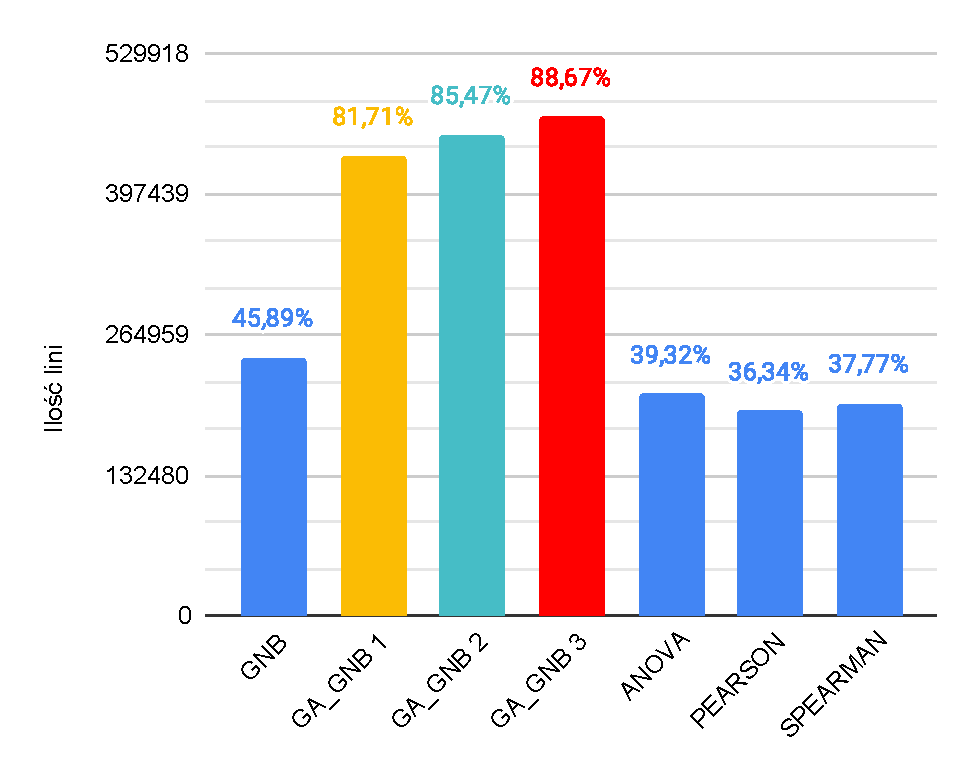
\includegraphics[width=0.7\textwidth]{images/Monday-WorkingHours_cmp}
    \captionsource{Klasyfikacja zbioru danych: Monday-WorkingHours}{\cite{Blyszcz2022}}
    \label{fig:mond}
\end{figure}

Analizując powyższe wyniki można zauważyć, że najwyższe dopasowanie uzyskał autorski algorytm a najniższe - zbiór kolumn wyznaczonych metodą współczynników korelacji Pearsona.\ Świadczy to o wysokiej jakości, opracowanego w pracy inżynierskiej, algorytmu.


\chapter{Sztuczna inteligencja}
Według słownika \textit{Oxford English Dictionary} słowo ''\textbf{inteligencja}'' oznacza zdolność do rozumienia, a analizy i dostosowania się do zmian\cite{OxfordJuly2023}.
\\ \\
Sztuczna inteligencja\trans{ang. Artificial Intelligence} (\textbf{AI}) jest wykorzystywana na wiele sposobów podczas prowadzenia badań naukowych: od stawiania hipotez oraz budowania twierdzeń matematycznych, tworzenia i monitorowania badań, zbierania danych i wielu innych czynności towarzyszącymi podczas badań. Najpopularniejszymi zastosowaniami jest między innymi uczenie nienadzorowane oraz wykrywanie anomalii\cite{AiScience, Mahesh2018}. Schemat podziału sztucznej inteligencji pokazano na \refsource{obrazie}{fig:si-schema}.

\begin{figure}[H]
    \centering
    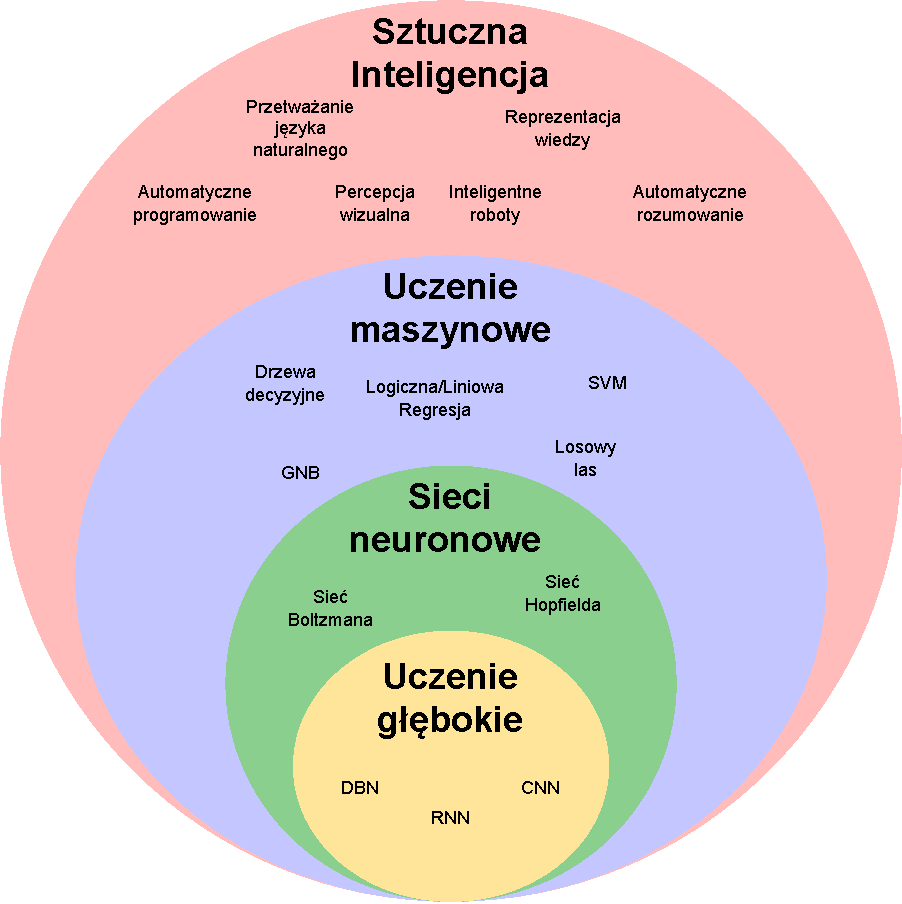
\includegraphics[width=0.5\textwidth]{images/si}
    \captionsource{Graficzne przedstawienie podziałów sztucznej inteligencji}{\cite{LinkedInSi}}
    \label{fig:si-schema}
\end{figure}

\section{Uczenie maszynowe}
Uczenie maszynowe\trans{ang. Machine Learning} (\textbf{ML}) jest to dziedzina nauki nad algorytmami oraz modelami statystycznymi, które mogą być wykorzystywane do specyficznych zadań na przykład klasyfikacji, rozpoznawania obrazów bądź mowy, a dodatkowo nie są zaprogramowane specyficznie pod konkretne zadanie, a jedynie pod grupę zadań tak jak pokazano na \refsource{obrazie}{fig:ml-schema}. Dlatego też nie ma jednego najlepszego rozwiązania, które można wykorzystać w każdym przypadku. Wykorzystanie konkretnego algorytmu determinuje typ zadania jaki ma być rozwiązany.

\begin{figure}[H]
    \centering
    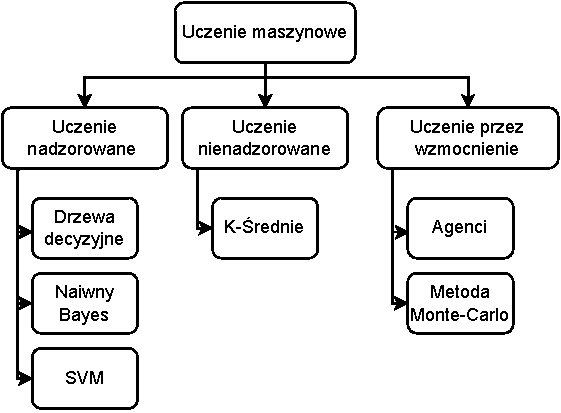
\includegraphics[width=\textwidth]{images/ml-przyklady}
    \captionsource{Podział uczenia maszynowego}{\cite{Mahesh2018}}
    \label{fig:ml-schema}
\end{figure}
    \subsection{Uczenie nadzorowane} - w trakcie tego uczenia stosuje się zbiór posiadający etykiety. Model uczy się przyporządkowywać określone cechy do konkretnych kategori. Dane wejściowe dzielone są na dane treningowe i dane testowe. Zbiór treningowy jest wykorzystywany do trenowania modelu, a zbió testowy do sprawdzenia rezultatu, na bazie którego może nastąpić korekta uczeniam zilustrowano to \refsource{obrazem}{fig:spervised}. Algorytmy uczenia nadzorowanego można zastosować między innymi do weryfikacji ruchu sieciowego w celu określenia czy ruch bezpieczny, przez co można to zastosować w systemach wykrywania intruzów\trans{ang. Intrusion Detection System} (\textbf{IDS}). Algorytmy wchodzące w skład uczenia nadzorowanego to między innymi klasyfikacja naiwna bayesa, drzewa decyzyjne, maszyny wektorów nośnych\cite{AiScience, Mahesh2018}.
    \begin{figure}[H]
        \centering
        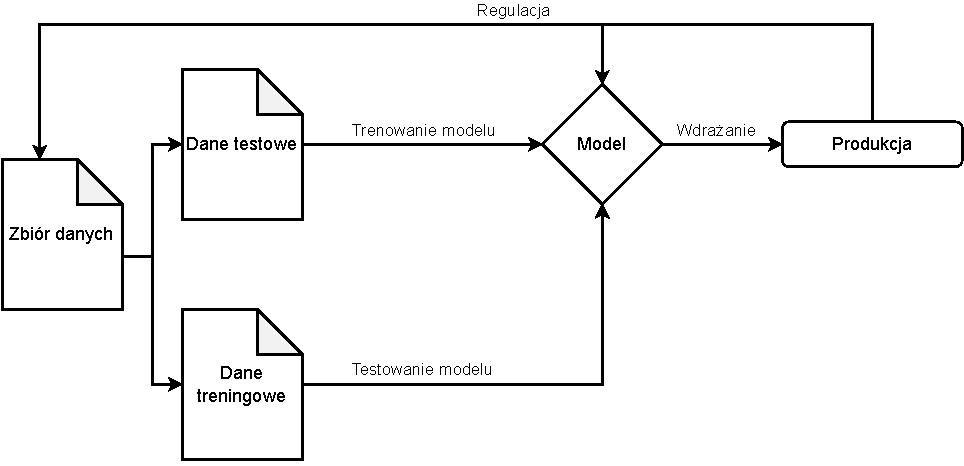
\includegraphics[width=0.75\textwidth]{images/supervised}
        \captionsource{Uczenie nadzorowane}{\cite{Mahesh2018}}
        \label{fig:spervised}
    \end{figure}

    \subsection{Uczenie nienadzorowane} - w tym przypadku nie wykorzystuje się zbioru oznaczonego, algorytm sam próbuje odkryć prawidłową odpowiedź. Dzieję się tak, w danych, których nie da się nazwać albo doprecyzować. Wykorzystuje się to do między innymi detekcji anomalii, co pozwoli do na przykład wykrycia zbyt dużego zużycia prądu w pokoju domu studenckiego dzieki czemu uda się wyłapać nieautoryzowaną koparkę kryptowalut. Dodatkowo można wykorzystać je do szukanai wzorców, albo zarządzania magazynem. W skład takich algorytmów wchodzi: K-średnie, klasteryzacja. Schemat uczenia nienadzorowanego poprzez klasteryzację jest pokazany na \refsource{obrazie}{fig:unspervised}.

    \begin{figure}[H]
        \centering
        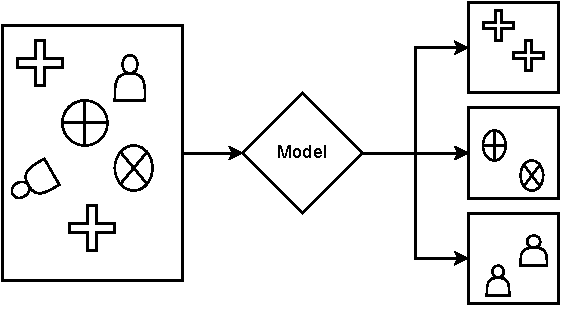
\includegraphics[width=0.5\textwidth]{images/unsupervised}
        \captionsource{Uczenie nienadzorowane}{Opracowanie własne}
        \label{fig:unspervised}
    \end{figure}

    \subsection{Uczenie przez wzmocnienie} - jest to uczenie poprzez nagradzanie dobrych rozwiązań, a karanie złych, potocznie mówiąc jest to metoda ''\textit{kija i marchewki}''. Wykorzystywana w trenowaniu pojazdów autonomicznych pozwala na nagradzanie pojazdów za wybór lepszych tras przykładowo za wybór dróg asfaltowych zamiast polnych. Skupia się w dużym stopniu na agencie i jego decyzjach w danym środowisku co pokazano na \refsource{schemacie}{fig:reinforcemenet}. Należy do jednych z trzech głównych paradygmatów obok uczenia nadzorowanego i nienadzorowanego.

    \begin{figure}[H]
        \centering
        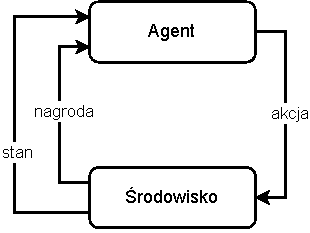
\includegraphics[width=0.5\textwidth]{images/reinforcemen}
        \captionsource{Uczenie przez wzmocnienie}{\cite{Mahesh2018}}
        \label{fig:reinforcemenet}
    \end{figure}

    \subsection{Uczenie częściowo nadzorowane} - do trenowania takich modeli stosuje się niewielkie zbiory oznaczone, oraz większe zbiory nieoznaczone, dzięki którym można próbować rozpoznać rozległe zbiory danych na podstawie pewnych cech wspólnych. Stosuje się to ze względu na mnogość danych na świecie, których opisanie byłoby niemożliwe oraz albo zbyt kosztowne. Przykładowo można znaleźć zastosowanie tych algorytmó w bankowości albo klasyfikowaniu stron internetowych poprzez wyszukiwanie treści na stronie i kategoryzowaniu ich\cite{semiLinkedin}. Jest to połączenie uczenia nadzorowanego i nienadzorowanego\cite{Mahesh2018}.

\section{Sieć neuronowa}
\label{sec:snn}
Ludzki mózg jest najbardziej złożonym organem znany ludziom. Badacze zainspirowani jego strukturą składającą się z połączonych ze sobą komórek neuronowych, które przetwarzają równolegle wiele informacji, próbują przenieść pewien poziom inteligencji do komputerów. Przykładem tego jest wiele algorytmów, wchodzących w skład sztucznych sieci neuronowych\trans{ang. artificial neural network} (\textbf{ANN}), między innymi sieci Kohonena, sieci Hopfielda, sieci konwolucyjne. Sieci te próbują w pewien sposób odwzorować próbę na przykład klasyfikacji danych przez jednostkę wzorowaną na ludzkim mózgu, pomimo tych osiągnięć symulacja ludzkiej świadomości oraz emocji wciąż jest jedynie w sferach fantazji naukowych\cite{Wang2003}.
\\ \\
Sieć neuronowa jest zbudowana z połaczonych ze sobą warstw neuronów tak jak na \refsource{rysunku}{fig:neural-network}, które w pewien sposób mają wykonać zadania uczenia maszynowego. Najprostszym przykładem sieci neuronowej jest pojedynczy neuron, który może służyć do prostych zadań klasyfikacyjnych: \refsource{schemat}{fig:neuron}. Sieć ta potrafi się dostosowywać do danych wejściowych tak aby uzyskać odpowiedni wynik, wykonuje w tedy proces uczenia stosując do tego na przykład algorytm wstecznej propagacji wag. W zależności od problemu istnieje wiele różnych sieci, które można zastosować. Jednym z trudniejszych rzeczy w doborze sieci jest dobór warstw ukrytych oraz ilości neuronów, ponieważ w tym celu twórca możę opierać się jedynie na własnej wiedzy i doświadczeniu. Podstawy teorii sieci neuronowych zostały stworzone w połowie XX wieku. Złota era uczenia maszynowego rozpoczęła się dopiero na początku XXI wieku, kiedy to jednocześnie pojawiły się takie trendy jak: Big Data, redukcja kosztów obliczeń równoległych, oraz pierwsze badania nad głębokimi sieciami neuronowymi\trans{ang. Deep Neural Network} (\textbf{DNN}). Największe zastosowanie DNN miało miejsce dopiero w ostatniej dekadzie kiedy to pojawiły się:
\begin{itemize}
    \item \textbf{Google Braine} - grupa badawcza założona w 2011 roku, zajmująca się badaniami nad sztuczną inteligencja
    \item \textbf{DeepFace} - rozwiązanie stworzone przez firmę Facebook w 2014 roku, służące do rozpoznawania twarzy na zdjęciu \cite{Koch2022, Fradkov2020}.
\end{itemize}

\begin{figure}[H]
    \centering
    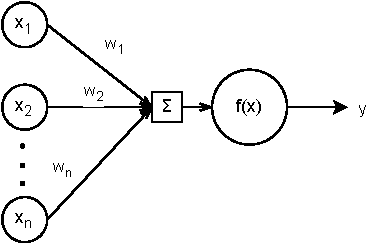
\includegraphics[width=0.5\textwidth]{images/neuron}
    \begin{itemize}
        \item[] $\Sigma$: sumator
        \item[] $f(x)$: funkcja aktywacyjna
        \item[] $w_x \  \forall x \in [1, 2, ..., n]$: wagi
        \item[] $x_x \  \forall x \in [1, 2, ..., n]$: wejścia
    \end{itemize}
    \captionsource{Schemat neuronu}{Opracowanie własne}
    \label{fig:neuron}
\end{figure}

\begin{figure}[H]
    \centering
    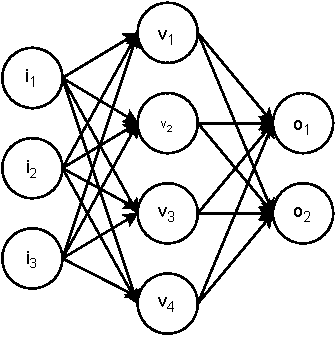
\includegraphics[width=0.75\textwidth]{images/neural-network}
    \begin{itemize}
    \item[] $i_x \ \forall x \in [1, 2, 3]$: dane wejściowe
    \item[] $v_x \ \forall x \in [1, 2, 3, 4]$: neurony w warstwie ukrytej
    \item[] $o_x \ \forall x \in [1, 2]$: dane wyjściowe
    \end{itemize}
    \captionsource{Schemat sieci neuronowej}{Opracowanie własne}
    \label{fig:neural-network}
\end{figure}

Sieci neuronowe możemy podzielić na wiele rodzajów, do których możemy zaliczyć między innymi:
\begin{itemize}
    \item \textbf{perceptron} - jest to najstarszy przykład sieci neuronowej złożonej z jednego perceptronu (neuronu). Można je zastosować w problemach klasyfikacji;
    \item \textbf{sieci wielowarstwowe perceptronowe} - jest to sieć złożona z wielu warstw połączonych ze sobą neuronów, najprostszy model sieci zaprezentowany na \refsource{rysunku}{fig:neural-network}. Składa się z warstwy wejściowej, warstw (jednej bądź wielu) ukrytych oraz warstwy wyjściowej. W neurony w tej sieci w porównaniu do perceptronów, mają funkcję aktywacyjną sigmoidalną, ze względu na rozwiązywanie problemów nieliniowych (posiadających więcej rozwiązań niż dwa 0/1). Można je zastosować na przykład do klasyfikacji danych;
    \item \textbf{sieci konwolucyjne (CNN)} - są to sieci służące do rozpoznawania obrazów, nazwa wzięła się od wykonywanej na obrazie operacji konwolucji (splotu). Sieci te posiadają dodatkowe warstwy konwolucyjne oraz spłaszczania, które pozwalają zamienić reprezentację obrazu w pojedyncz;
    \item \textbf{sieci rekurencyjne} - charakteryzują się pętlą zwrotną w warstwie ukrytej. Mogą być wykorzystane do generowania tekstu, tłumaczen maszynowych, a także na przykład przewidywania cen rynkowych;
    \item \textbf{sieci samoorganizujące się} - wykorzystuje uczenie nienadzorowane oraz. Składają sie jedynie z warstwy wejściwej i wyjściowej. Zaś cechą charakterystyczną jest to, że neurony określające podobne klasy znajdują się obok siebie. Sieci te mogą być wykrozystywane do podziału klientów na odpowiednie grupy bądź do wskazania jakim klientom zaproponować karty kredytowe \cite{IBMNetwork, BartosSOM}.
\end{itemize}

\subsection{Głębokie uczenie}
Jest to podkategoria uczenia maszynowego polegająca na tworzeniu wielowarstwowych sieci neuronowych. W porównaniu do podstawowych sieci neuronowych potrzebuje ogromnych zbiorów danych do utworzenia modelu predykcyjnego. Potrzebuje również dużo więcej mocy obliczeniowej przez wzgląd na ilość warstw ukrytych, których może być dużo więcej, przykładem najprosztszej sieci głębokiej jest \refsource{obraz}{fig:deep-learn}.

\begin{figure}[H]
    \centering
    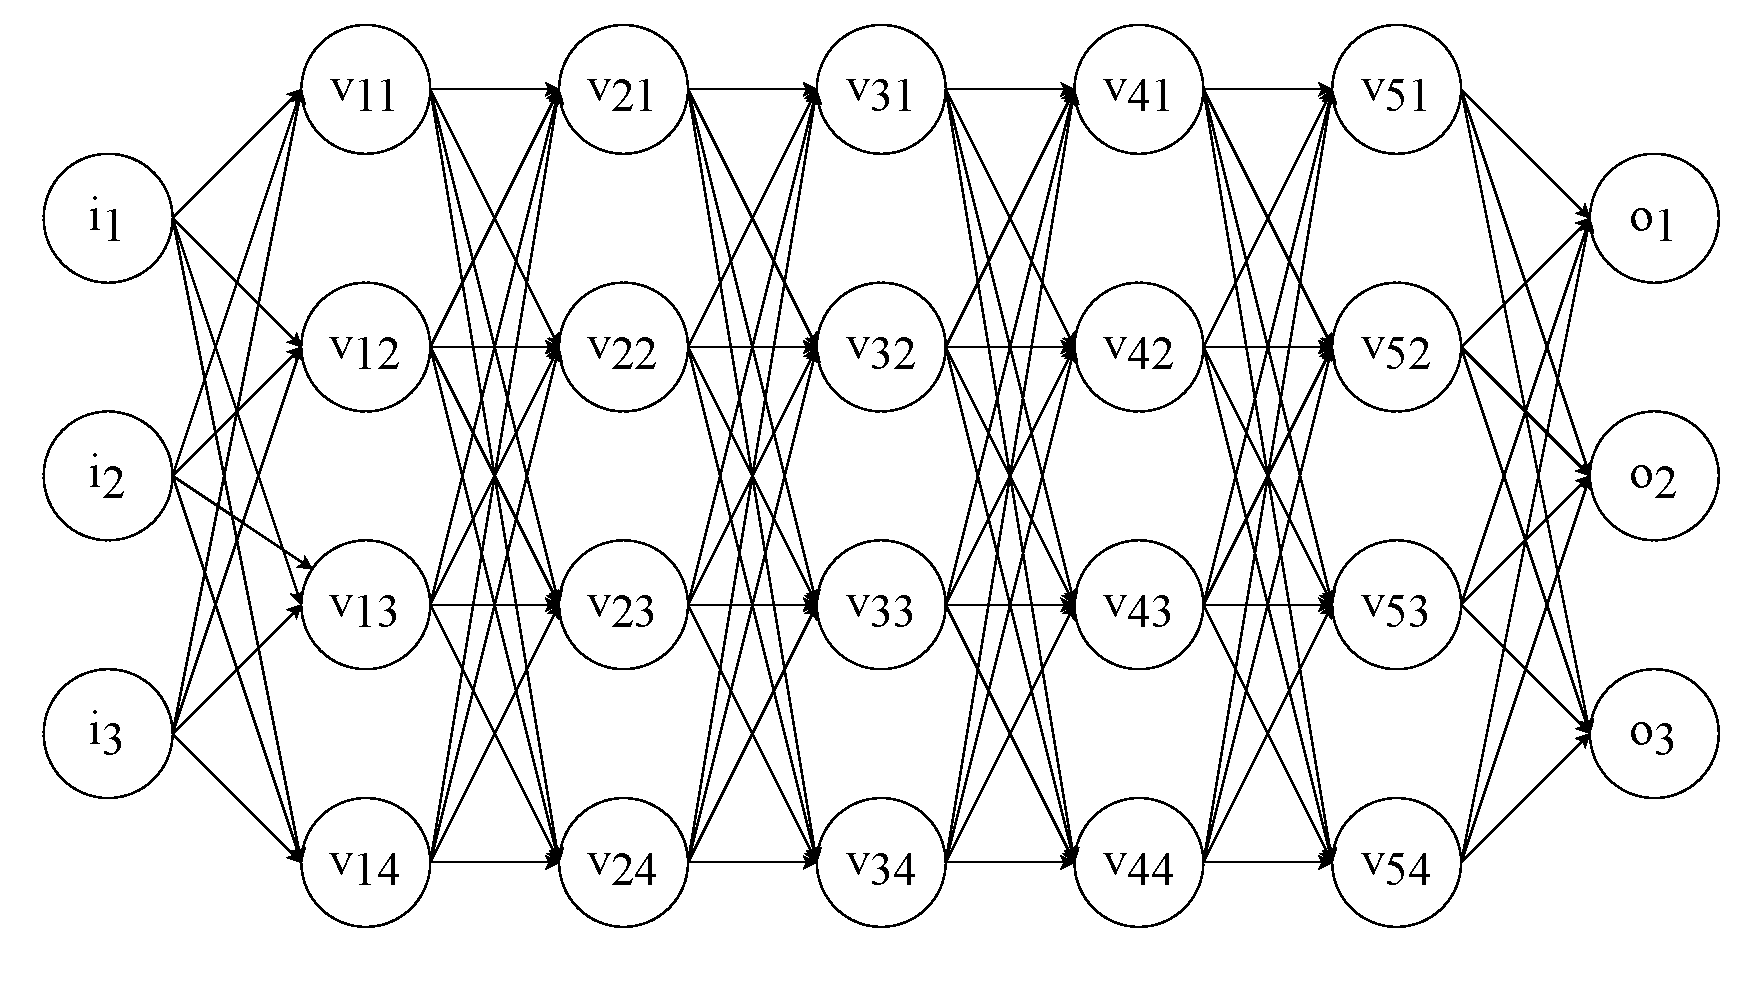
\includegraphics[width=0.75\textwidth]{images/deep-neural-network}
    \begin{itemize}
        \item[] $i_x \  \forall x \in [1, 2, 3]$: dane wejściowe
        \item[] $v_x \ \forall x \in [11, 12, 13, 21, 22, 23, 31, 32, 33]$: neurony w warstwie ukrytej
        \item[] $o_x \ \forall x \in [1, 2]$: dane wyjściowe
    \end{itemize}
    \captionsource{Schemat prostej głębokiej sieci neuronowej}{Opracowanie własne}
    \label{fig:deep-learn}
\end{figure}

Warstwa wyjściowa DNN może dostarczać dane róznego formatu, może to być na przykłąd, tekst, liczba bądź dźwięk. Posiada również bardzo dużo zastosowań w któych skład wchodzi generowanie treści, Deepfake, analiza obrazów, wskazywanie obiektów na obrazach, projektowanie leków, czatboty. Jest to udoskonalenie podstawowych sieci neuronowych. Tak więc częśc typów sieci opisanych w \refsource{sekcji}{sec:snn} będzie odnosić się do głębokich sieci neuronowych, należy do nich CNN\cite{MicrosoftDepp2023}.
\chapter{Klasyfikacja danych}

 Człowiek od zawsze próbuje skategoryzować i uporządkować posiadaną wiedzę w zbiory pozwalające na łatwy dostęp do przechowywanych informacji na przykład w sposób tabelaryczny. Klasyfikacja to proces rozpoznawania obiektów na bazie analizy ich cech. Jest to jedna z pierwszych rzeczy, której uczą się niemowlęta: rozróżniania kształtów, kolorów czy własnych rodziców. \ W póżniejszych latach te umiejętności są bardzo ważne, ponieważ w otaczającym świecie wiele rzeczy jest sklasyfikowanych. Przykładem takiej klasyfikacji są książki w katalogach bibliotecznych czy produkty spożywcze według jakości produkcji.
\\ \\
W uczeniu maszynowym klasyfikacja jest to metoda uczenia nadzorowanego, podczas której model próbuje przewidzieć etykietę obiektu na podstawie jego cech. Proces uczenia modelu klasyfikacji jest oparty o dwa zbiory, treningowy i testowy. Zbiór treningowy powinien być mniejszy od zbioru testowego. Po udanym procesie trenowania modelu następuje proces testowania, na podstawie którego wylicza się odpowiednie metryki pozwalające na ewaluacje modelu. W pracy magisterskiej wykorzystano zbiór danych, który posiada dwa typy etykiet [0, 1], dlatego też na tej podstawie zbudowano macierz pomyłek.

\section{Metryki klasyfikacji danych}
W trakcie ewaluacji algorytmu służącego do klasyfikacji wykorzystuje się metryki klasyfikacji. Służą one do przewidywania etykiet klas na podstawie danych wejściowych. W zależności od ilości klas wyjściowych rozróżniamy klasyfikację binarną i wieloklasową. W klasyfikacji binarnej występują tylko dwie klasy wyjściowe, a w klasyfikacji wieloklasowej już tych klas jest więcej. Przykładem klasyfikacji binarnej jest np. wykrywanie niechcianych wiadomości w skrzynce mailowej. Wiadomość przychodzącą możemy określić jako 1 - \textit{,,pozytywną''}, bądź 0 - \textit{,,negatywną''}. Istnieje wiele sposobów na oceny klasyfikacji, do których zaliczamy między innymi dokładność, macierz pomyłek czy precyzję~\cite{Agrawal2024}.
\\ \\
Macierz pomyłek pokazuje jakie wyniki możemy otrzymać w procesie klasyfikacji. \refsource{Tabela}{tab:matrix-tn} obrazuje schemat macierzy pomyłek. Jest to miara wydajności problemów klasyfikacji.

\begin{table}[H]
    \centering
    \captionsource{Macierz pomyłek}{Opracowanie własne}
    \label{tab:matrix-tn}
    \begin{tabular}{|c|c|M{16mm}|M{16mm}|}
        \hline
         & & \multicolumn{2}{c|}{\textbf{Prawdziwe wartości}} \\ \hline
         & & \textbf{1} & \textbf{0} \\ \hline
        \rule{0pt}{13mm} \multirow{2}{*}{\rotatebox[origin=c]{90}{\parbox{18mm}{\textbf{Przewidziane wartości}}}} & \textbf{1} & \cellcolor{lightgreen}TP & \cellcolor{lightred}FN \\ \cline{2-4}
        \rule{0pt}{13mm} & \textbf{0} & \cellcolor{lightred}FP & \cellcolor{lightgreen}TN \\ \hline
    \end{tabular}
\end{table}
    Wyróżniamy 4 rodzaje rezultatów:
    \begin{itemize}
        \item  \textbf{TP} (\textit{prawdziwie pozytywny}) -- przewidywano pozytywny wynik i otrzymano pozytywny wynik,
        \item \textbf{FN} (\textit{fałszywie negatywny}) -- przewidywano negatywny wynik, a otrzymano pozytywny wynik,
        \item \textbf{FP} (\textit{fałszywie pozytywny}) -- przewidywano pozytywny wynik, a otrzymano negatywny wynik,
        \item \textbf{TN} (\textit{prawdziwie negatywny}) -- przewidywano negatywny wynik i otrzymano negatywny wynik.
    \end{itemize}

Opierając się o macierz pomyłek można wyznaczyć następujące metryki:
\begin{itemize}
    \item dokładność,
    \item precyzję,
    \item czułość,
    \item F1
    \item swoistość
    \item ROC-AUC~\cite{Agrawal2024}
\end{itemize}

\subsection{Dokładność}
\begin{equation}\label{math:acc}
    \frac{TP + TN}{TP + TN + FP + FN}
\end{equation}
Dokładność określa częstość poprawnego przewidywania klasyfikatora. Jest to stosunek wszystkich dobrze oznaczonych obiektów do liczby wszystkich prób~\cite{Agrawal2024, Blyszcz2022, Kulkarni2020}.

\subsection{Precyzja}
\begin{equation}\label{math:prec}
    \frac{TP}{TP + FP}
\end{equation}
Precyzja wyjaśnia ile z prawidłowo przewidzianych przypadków jest poprawnych. Jest to stosunek poprawnie wybranych obiektów klasy ,,\textit{1}'', do wszystkich wybranych obiektów tej klasy. Znajduje zastosowanie w przypadkach gdy wynik fałszywie dodatni jest większym problemem niż fałszywie ujemny~\cite{Agrawal2024, Blyszcz2022, Kulkarni2020}.

\subsection{Czułość}
\begin{equation}\label{math:rec}
    \frac{TP}{TP + FN}
\end{equation}
Czułość określia ile rzeczywistych pozytywnych przypadków byliśmy w stanie poprawnie przewidzieć za pomocą naszego modelu. Jest to stosunek poprawnie sklasyfikowanych obiektów klasy ,,\textit{1}'', do wszystkich obiektów, które powinny być w tej klasie. Czułość jest przydatną metryką w przypadkach gdy wynik fałszywie ujemny ma większe znaczenie niż wynik fałszywie dodatni~\cite{Agrawal2024, Blyszcz2022, Kulkarni2020}.

\subsection{Swoistość}
\begin{equation}\label{math:swo}
    \frac{TN}{TN + FP}
\end{equation}
Swoistość lub specyficzność pozwala określić ile rzeczywiście uzyskało się przypadków negatywnych. Jest to stosunek poprawnie zaklasyfikowanych obiektów klasy ,,\textit{0}'', do wszystkich obiektów, które powinny być w tej klasie~\cite{Agrawal2024}.

\subsection{F1}
\begin{equation}\label{math:f1}
   \frac{2*x*y}{x + y}
\end{equation}
Parametr F1 pozwala na połączoną ocenę precyzji i czułości. Jest to średnia harmoniczna precyzji (\textit{x}) i czułości (\textit{y}). Parametr F1 może być skuteczną metryką oceny w następujących przypadkach:
\begin{itemize}
    \item wyniki fałszywie pozytywne i fałszywie negatywne są równie kosztowne
    \item zwiększenie ilości danych nie zmienia skuteczności wyniku
    \item wynik prawdziwie ujemny jest wysoki~\cite{Agrawal2024}.
\end{itemize}

\subsection{ROC - AUC}
Krzywa ROC-AUC przedstawiona na \refsource{rysunku}{fig:roc-auc}, pozwala na ocenę sprawności klasyfikatora. ROC jest krzywą prawdopodobieństwa, którą wykreśla czułość w stosunku do swoistości. Wykres przedstawia wydajność (dokładność predykcji) modelu klasyfikacji. AUC \textit{(ang. Area Under Roc Curve)} jest to pole pod krzywą ROC. AUC to miara zdolności klasyfikatora do rozróżniania klas.

\begin{figure}[H]
    \centering
    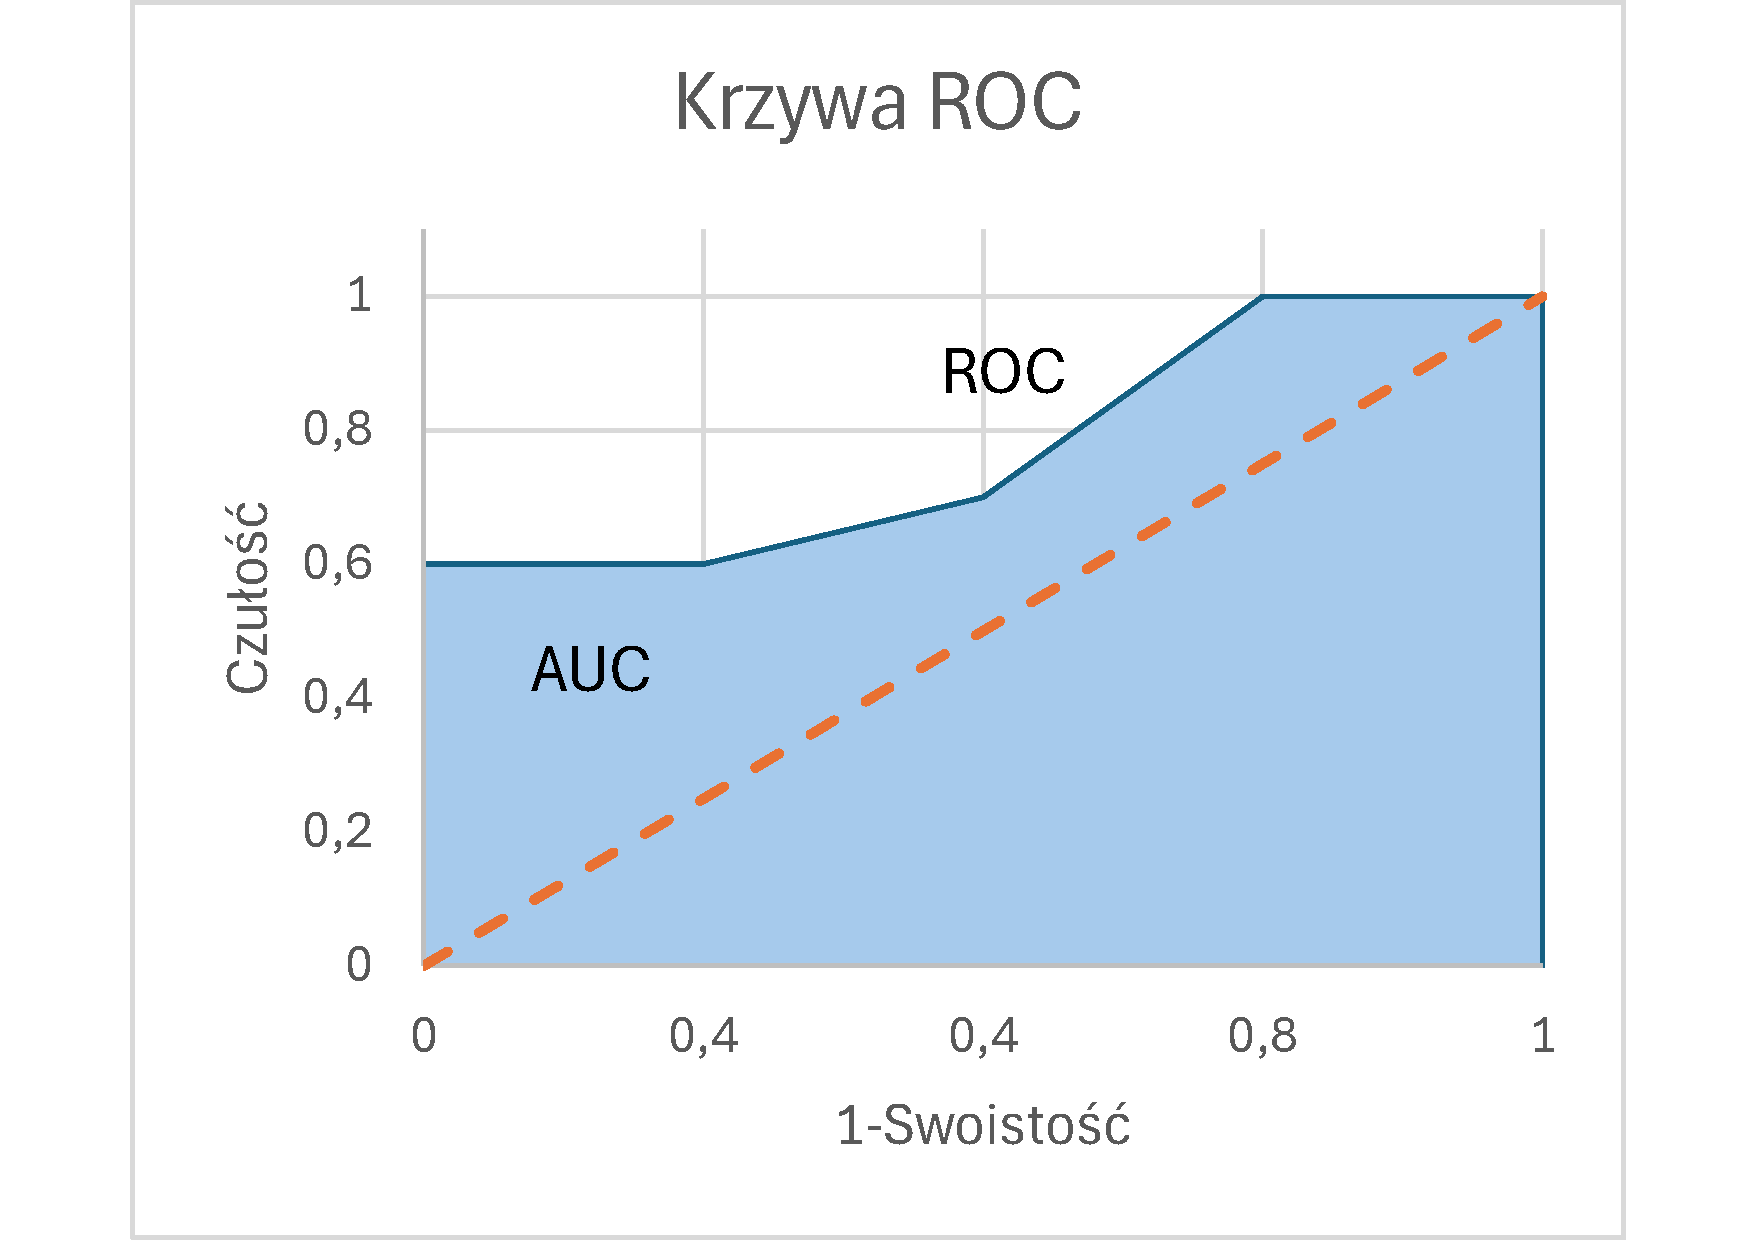
\includegraphics[width=0.8\textwidth]{images/roc-auc}
    \captionsource{Przykład krzywej ROC}{Opracowanie własne}
    \label{fig:roc-auc}
\end{figure}

Im większa jest wartość AUC tym lepsza wydajność modelu w rozróżnianiu klas pozytywnych i negatywnych. Wynik AUC jest z zakresu $[0, 1]$:
\begin{itemize}
    \item AUC = 1 -- klasyfikator idealny, który rozróżnia wszystkie punkty,
    \item 0,5 < AUC < 1 -- klasyfikator prawie idealny, czyli z dużym prawdopodobieństwem sklasyfikuje poprawnie obiekty
    \item AUC = 0,5 -- klasyfikator losowy, oznacza to, że nie ma pewności czy klasyfikator jest w stanie rozpoznać cechy, czy może przypisuje je losowo,
    \item AUC < 0,5 -- klasyfikator gorszy niż klasyfikator losowy~\cite{Algolytics, Agrawal2024}.
\end{itemize}
\chapter{Podejście low-code/no-code}
Low-Code oraz no-code to nowe podejście skupiające się na umożliwieniu tworzenia programów w sposób nie wymagający znajomości języka oprogramowania. Podejście to ma pozwolić osobom nie będącymi programistami na tworzenie aplikacji biznesowych. Ma to zwiększyć tempo tworzenia rozwiązań biznesowych, na które zapotrzebowanie wciąż rośnie. Jednakże podejście to jest stosounkowo świeżym podejściem, którego początki można było obserwować w codziennym życiu na przykład podczas tworzenia stron internetowych korzystając z narzędzi takich jak \textit{Wordpress}, \textit{Joomla}, \textit{Wix}. Narzędzia te umożliwiają w łatwy sposób tworzyć stronę z tak zwanych kafelków, które umieszczone w odpowiednim miejscu były odpowiedzialne za jedną konkretną rzecz\cite{Wordpress2023, Joomla2023, Wix2023}. Przykład na \refsource{obrazie}{fig:pa-plat}, \textbf{\ref{fig:wp-plat}}.
\begin{figure}[H]
    \centering
    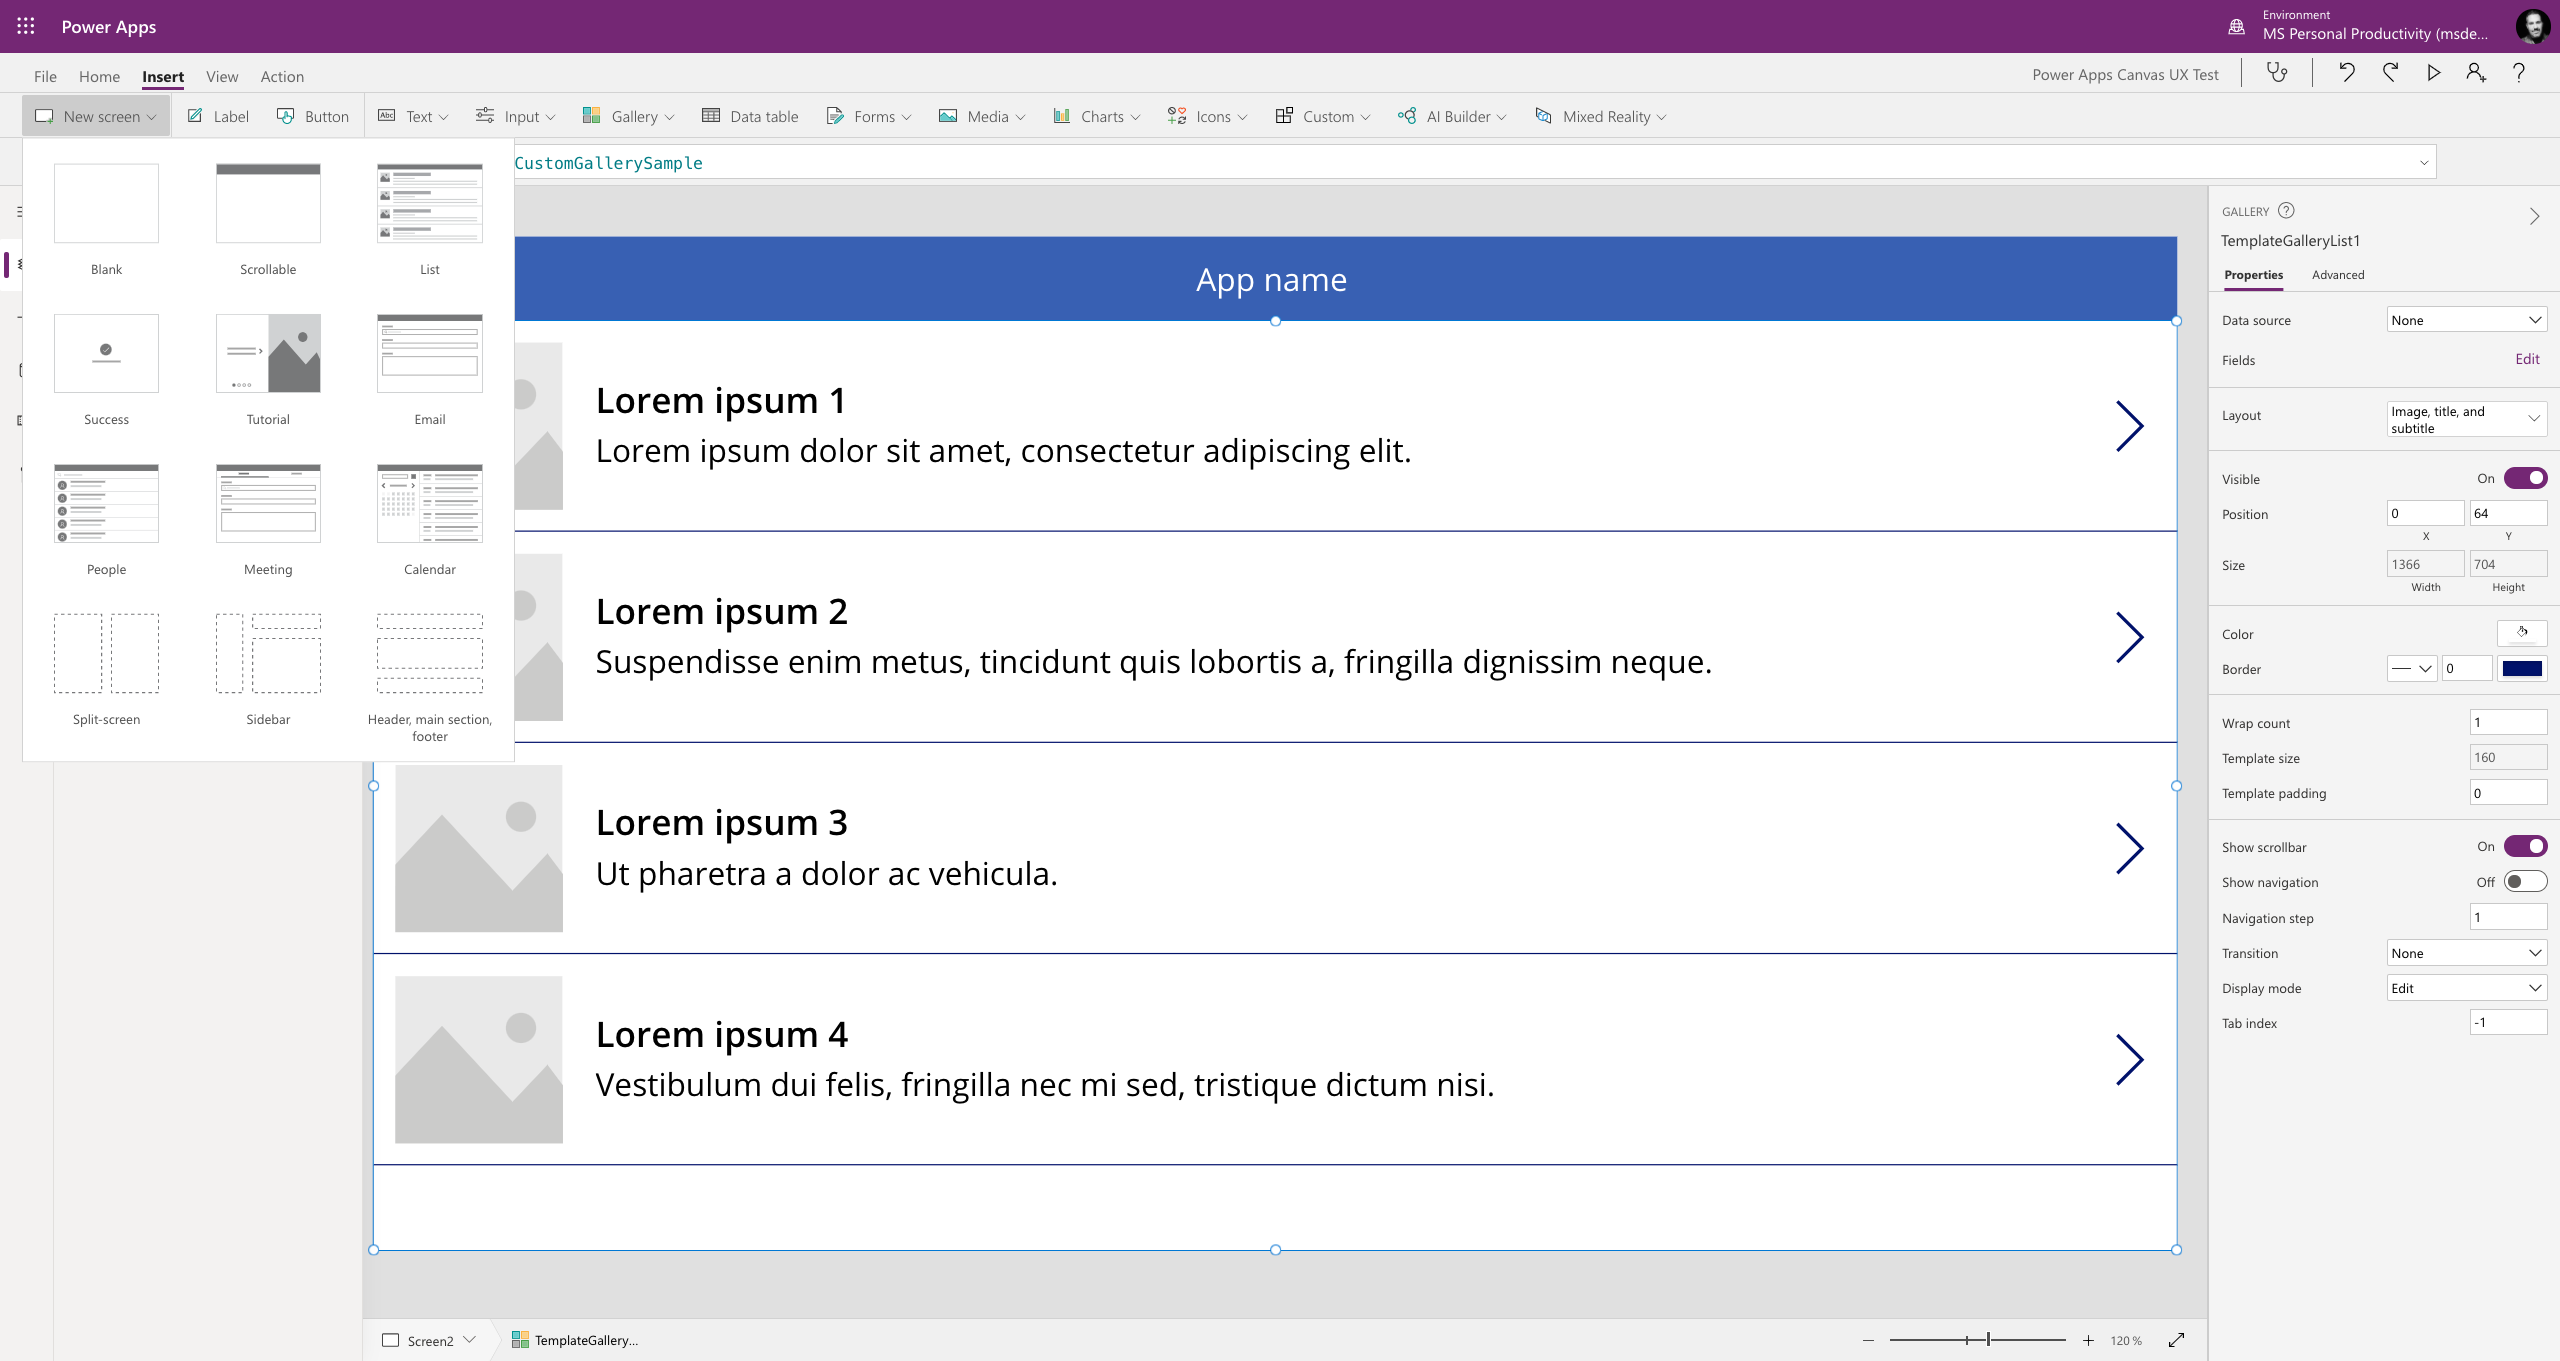
\includegraphics[width=0.6\textwidth]{images/ms_powerapps}
    \captionsource{PowerApps od Microsoft}{\cite{Powerapps2023}}
    \label{fig:pa-plat}
\end{figure}

\begin{figure}[H]
    \centering
    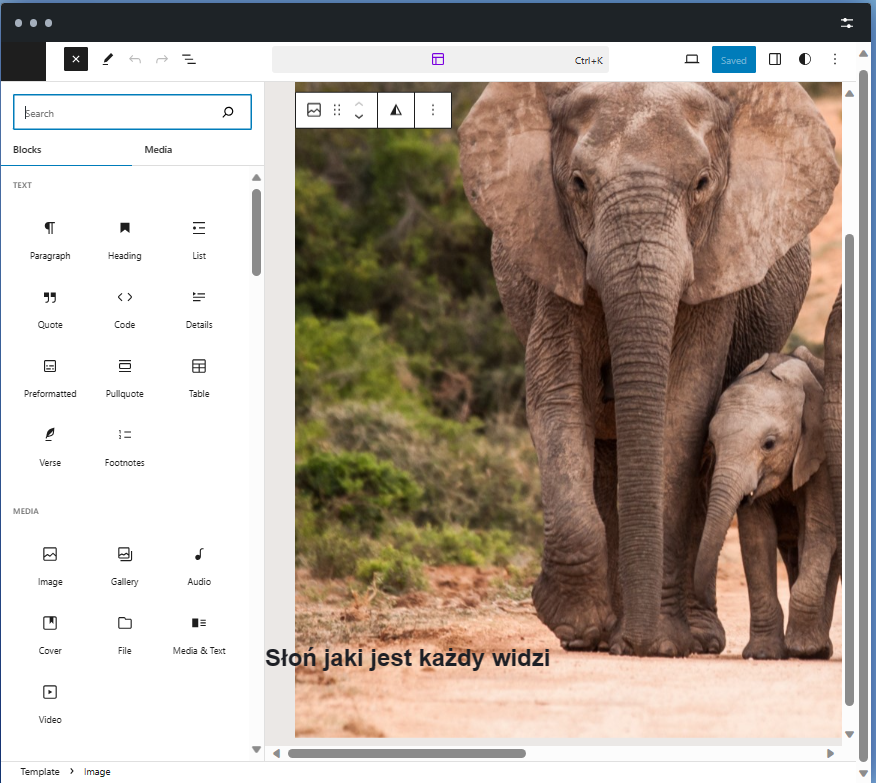
\includegraphics[width=0.4\textwidth]{images/slon_wordpress}
    \captionsource{Wordpress.com}{\cite{WordpressDeveloper2023}}
    \label{fig:wp-plat}
\end{figure}

Coraz większa popularnością cieszą się platformy low-code\trans{ang. Low-code Development Platforms} (\textbf{LCDPs}) dostarczane między innymi przez Google, Microsoft, Amazon pozwalają one na tworzenie wysoko skalowalnych rozwiązań przy niewielkim albo i żadnym nakładzie programowania. Ma to umożliwić osobom z niewielkim doświadczeniem w programowaniu, na szybkie wdrożenie oraz tworzenie niezawodnego oprogramowania. Twórcy platform oferują również korzystającym zmniejszenie ilości pracy potrzebnej do wdrożenia albo rozwijania kolejnych funkcjonalności\cite{Bock2021, Hirzel2022}.
\\ \\
\section{Platformy}
LCDP udostępniane twórcom aplikacji, umożliwiają skalowalność rozwiązań tworzonych na własne potrzeby. Dodatkowo są popularne przy tworzeniu aplikacji typu ''\textit{aplikacja jako usługa}'' \trans{ang. Software-as-a-Service} (SaaS), które opłacane są tylko za stopień ich użycia, co w niektórych przypadkach może się okazać dużo bardziej opłacalne niż utrzymywanie swoich rozwiązań serwerowych. Dzięki takim rozwiązaniom wiele małych firm będzie mogło pozwolić sobie na tworzenie i utrzymywanie dostosowanych rozwiązań opartych o ekosytem \textit{Microsoft365} / \textit{Google Workspace}.

\subsection{Microsoft PowerApps}
Jest to platforma programistyczna umożliwiająca tworzenie niestandardowych aplikacji dla rozwiązań biznesowych. Umożliwia ona tworzenie aplikacji opartych o różnorakie źródła danych do których należą między innymi: SQL Server, SharePoint, Dynamics 365. Dodatkową zaletą tego rozwiązania jest tworzenie aplikacji responsywnych, działających dobrze na wielu rodzajach urządzeń. Dodatkowow platforma ta pozwala tworzyć trzy typy aplikacji przy braku konieczności kodowania\cite{Microsoftc}
\begin{itemize}
    \item \textbf{Kanwa} - jest to typ aplikacji oparty o model danych znajdujący się na przykład w Excelu. Aplikację tego typu tworzy się za pomcą przesuwanych kafelek, a proces przypomina po trochu robienie prezentacji przy użyciu aplikacji Powerpoint, co umożliwia pełną dowolność w tworzonym interfejsie graficznym\cite{Microsoftb}.

    \item \textbf{Oparte na modelu} - w ramach korzystania z usługi Microsoft Dataverse można wygenerować aplikacje bazujące na danym modelu danych, przez co użytkownicy otrzymują produkt ułatwiający im analizę danych\cite{Microsofta}.

    \item \textbf{Karty} - są to uproszczone aplikacje, które można dodać do usługi Micrsoft Teams w określonym biznesowym celu. Dużą zaletą tego rozwiązania jest możliwość korzystania z źródeł danych, dzięki czemu poszczególne karty mogą odpowiadać za jedno zadanie biznesowe\cite{Microsoft}.
\end{itemize}

\subsection{Amazon QuickSight}
Jest to rozwiązanie firmy Amazon, które umożliwia firmom dostarczanie rozwiązań z zakresu analityki biznesowe\trans{ang. business intelligence} (BI) dzięki interaktywnym pulpitom korzystającym z jednego źródła prawdy. Dodatkowo korzystanie z interaktywnych formularzy, raportów oraz zapytań w języku naturalnym pozwala interesariuszom otrzymać możliwość korzystania z jednolitych rozwiązań opartych o różne modele danych\cite{AmazonQuickSight}.

\subsection{Google AppSheet}
Platforma AppSheet od firmy Google umożliwia tworzenie aplikacji mobilnych oraz desktopowych bez użycia kodu. Firma wskazuje na możliwości integracyjne z różnymi dostawcami danych, do których należą między innymi Microsoft, Dropbox, a także wbudowaną integrację z aplikacjiami Google Workspace do któych należą Gmail, Sheets oraz Spaces. Platforma pozwala również na tworzenie automatycznych botów, które wykonują zadania w oparciu o bodźce zewnętrzne bądź wewnętrzne. Narzędzie pozwala w prosty sposób na tworzenie szybkich rozwiązań biznesowych w oparciu o ekosystem firmy Google\cite{GoogleAppSheet}.



\chapter{Microsoft Azure}
Platforma została oddana do użytku w 2008 roku jako Windows Azure.\ Usługa ta została zbudowana na modułach Windows NT.\ Platforma została udostępniona komercyjnie po 2010 roku, kiedy to dodano możliwość korzystania z szerszej ilości usług i języków programowania.\ Do usług należało między innymi udostępnienie baz danych Microsoft SQL Server opartych o .NET Framework 4, obsługę aplikacji pisanych w wielu języku (takich jak \textit{C\#}, \textit{Java}, \textit{PHP}), sieć dostarczania zawartości \trans{ang. Content Delivery Network, CDN}.
\\ \\
Następnym krokiem było przemianowanie platformy na Microsoft Azure oraz pójście w kierunku infrastruktury definiowanej jako serwis \trans{ang. Infrastructure-as-a-Service, IaaS}, oraz powolne adoptowanie usług open-source.
\\ \\
W kolejnej generacji Microsoft zaadoptował rozwiązania Big Data do swojej platformy, umożliwiając korzystanie z języka \textit{R}, połączenie do Power BI, a także umożliwienie połączenia do rozwiązań end-to-end.
\\ \\
W czwartej generacji platformy, Microsoft skupił się na rozwiązaniach uczenia maszynowego oraz integracji z bazami danych, dzięki czemu powstało Azure Machine Learning Studio oraz Azure Machine Learning Operations (MLOps).
\\ \\
Obecnie platforma została wzbogacona o Kubernetesa, dzięki czemu konteneryzacja ułatwiła pracę z klastrami wirtualnymi.\ Wirtualne klastry pozwalają na wydajniejszy i wygodniejszy sposób zarządzania aplikacjami i usługami.\ Dodatkowo zostało udostępnione wiele kombinacji usług takich jak: aplikacja jako usługa \trans{ang. Software-as-a-Service} (SaaS), Interfejs jako usługa \trans{ang. Infrastucture-as-a-Service} (IaaS), Platforma jako usługa \trans{ang. Platfrom-as-a-Service} (PaaS).\ Microsoft uzyskał w ten sposób platformę przyjazną użytkownikowi, która umożliwia użytkownikom korzystanie z ponad 200 dostępnych usług.\ Dodatkowo płatność za platformę jest rozliczana tylko za zużytą przestrzeń oraz wykorzystaną moc obliczeniową~\cite{Roosevelt2022, MicrosoftAzurec, Datashift}.

\vfill
\pagebreak

\begin{figure}[H]
    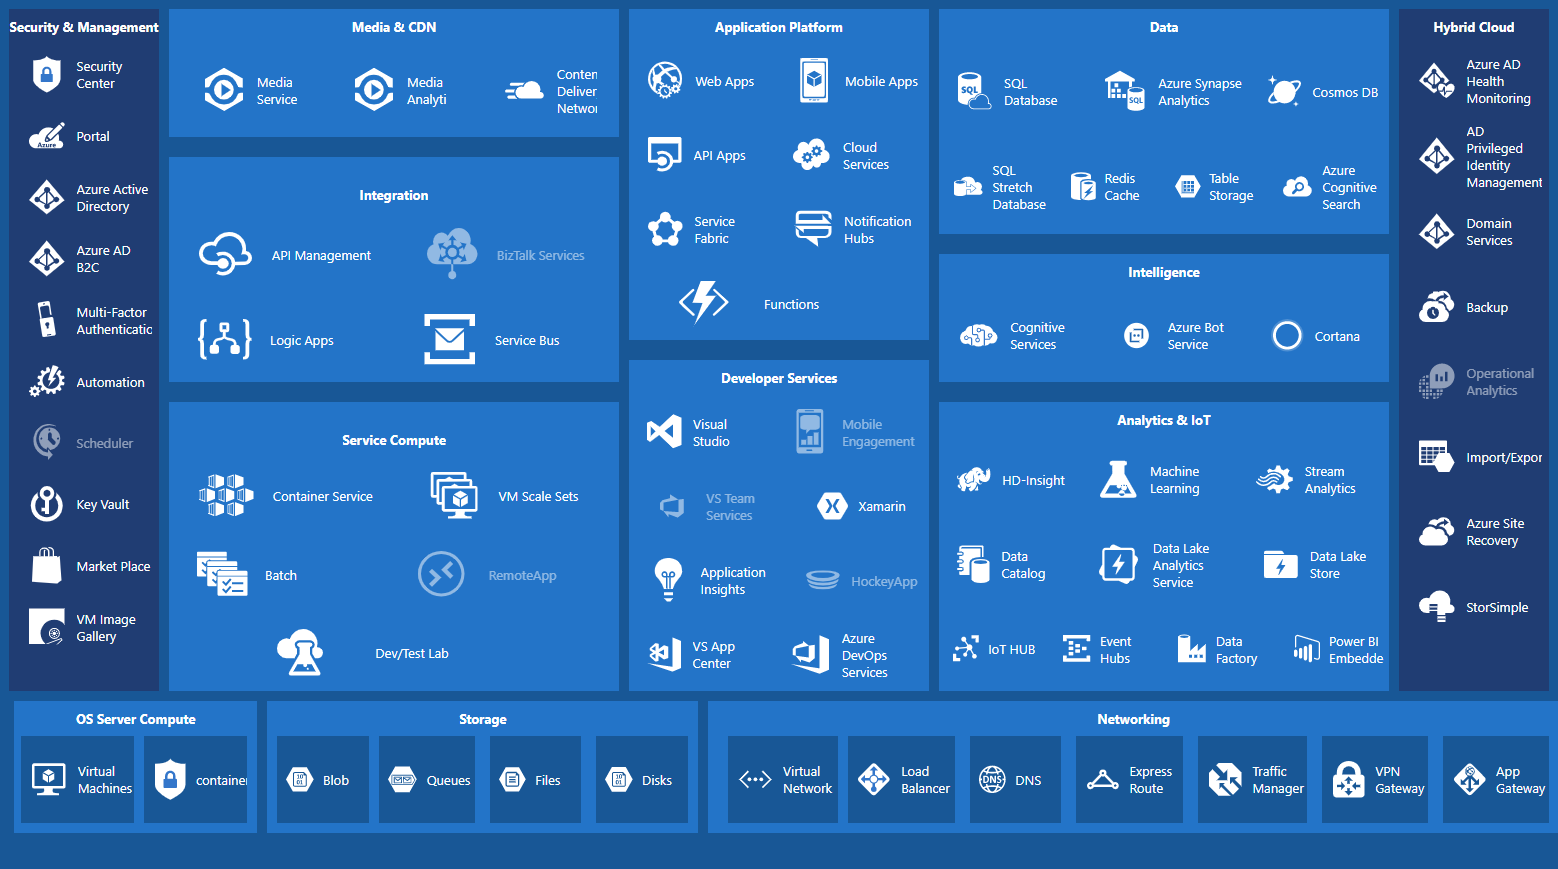
\includegraphics[width=\textwidth]{images/ms_azure}
    \captionsource{Schemat podziału usług MS Azure}{\cite{Datashifta}}
    \label{fig:ms-azure}
\end{figure}

\refsource{Schemat}{fig:ms-azure} pokazuje jak obecnie podzielone są usługi oraz co jest udostępnione komercyjnie w ramach platformy Azure.\ Według schematu platforma podzielona jest na trzynaście obszarów, do których zaliczono między innymi bezpieczeństwo, zarządzanie danymi, usługi deweloperskie, analiza danych, platformy aplikacji.

\section{Infrastruktura}
Infrastruktura globalna Azure składa się z dwóch części: fizycznej infrastruktury oraz globalnej łączności.\ Infrastruktura fizyczna składa się z ponad 200 centrów danych na całym świecie, połączonych w jedną globalną sieć.\ Takie rozwiązanie umożliwia wysoką skalowalność i dostępność poszczególnych rozwiązań.\ Cały ruch sieciowy jest utrzymywany wewnątrz prywatnej sieci Microsoft.\ Pozwala to na zachowanie informacje o adresach IP wewnątrz sieci, a co za tym idzie, informacje te nie trafiają do opinii publicznej~\cite{MicrosoftAzureb}.\\ \\

Na swojej stronie internetowej Microsoft udostępnia wirtualną mapę, umożliwiającą zobaczenie aktualnej sieci Microsoftu oraz jej rozmieszczenie na globie ziemskim.\ Interaktywna mapa pozwala uzyskiwać informację o poszczególnych krajach oraz centrach danych znajdujących się na terytoriach tych krajów.\ Mapę oraz informację pokazano na \refsource{zdjęciach}{fig:azure-ic}.

\vfill
\pagebreak

\begin{figure}[H]
    \begin{subfigure}[m]{0.7\textwidth}
    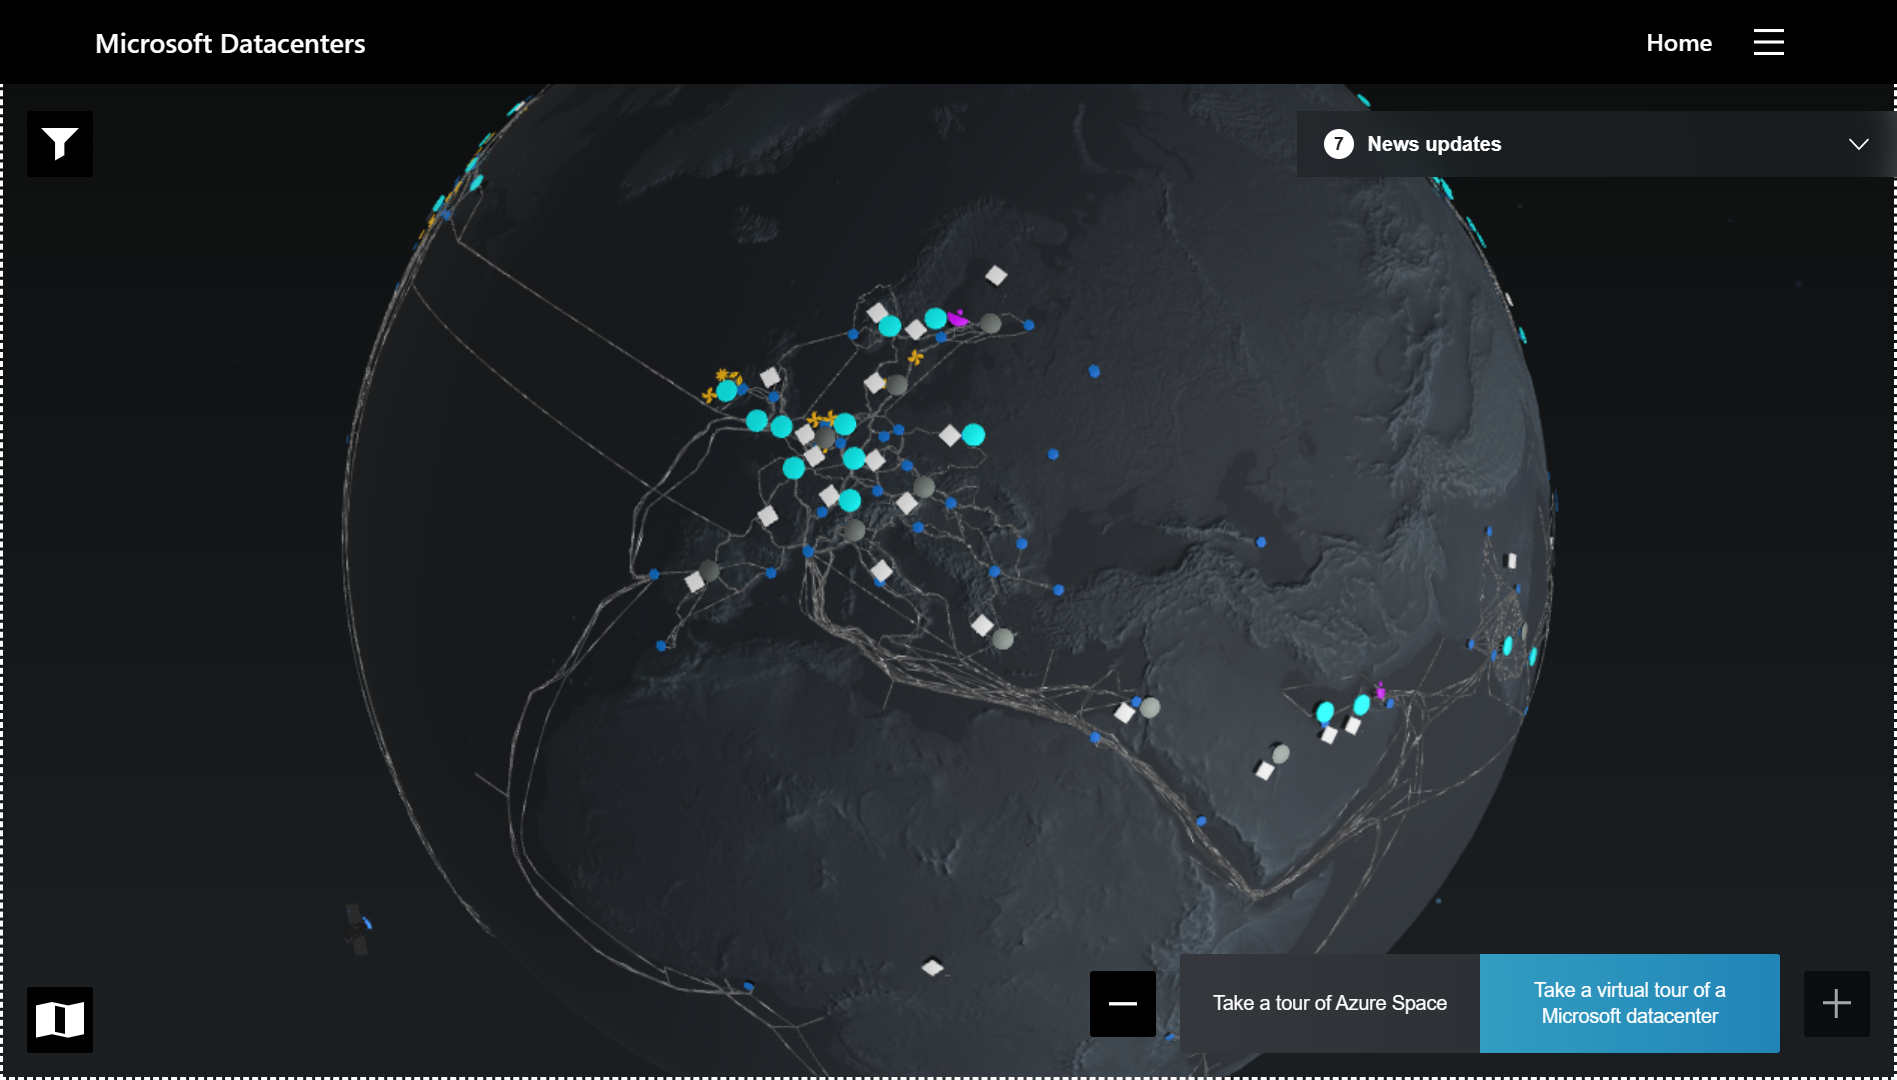
\includegraphics[width=\textwidth]{images/azure-ic}
    \captionsource{Globalna mapa infrastruktury sieciowe}{\cite{MicrosoftAzured}}
    \end{subfigure}
    \hfill
    \begin{subfigure}[m]{0.25\textwidth}
        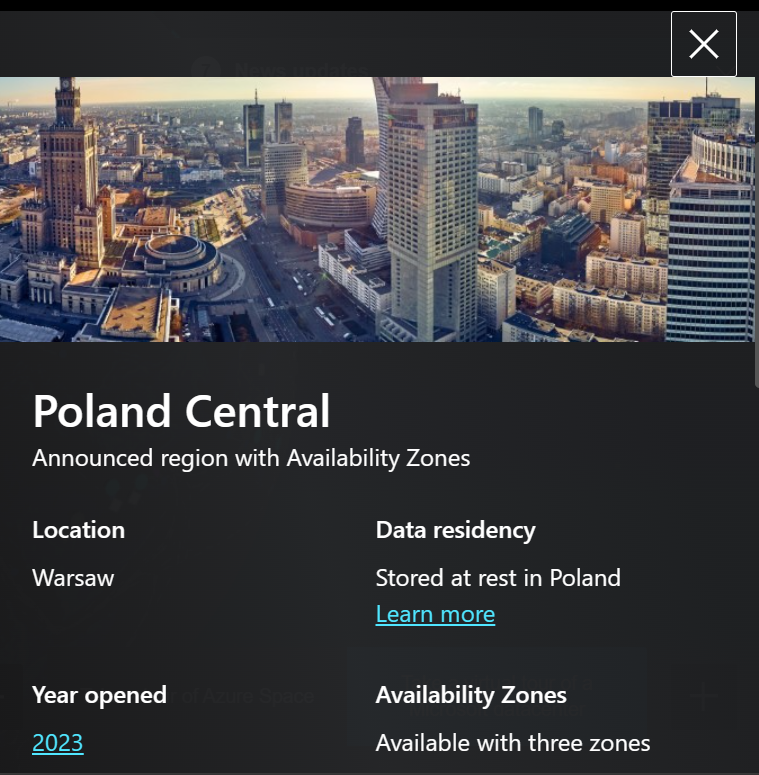
\includegraphics[width=\textwidth]{images/azure-pl}
        \captionsource{Informacje o centrum danych}{\cite{MicrosoftAzuree}}
    \end{subfigure}
    \captionsource{Zdjęcia z mapy insfrastruktury Microsoft Azure}{\cite{MicrosoftAzuree, MicrosoftAzured}}
    \label{fig:azure-ic}
\end{figure}

\section{Machine Learning Studio}
Azure Machine Learning Studio to platforma low-code.\ Umożliwia łatwe i szybkie tworzenie wysoce wydajnych modeli uczenia maszynowego, a także zarządzanie nimi.\ Użytkownik nie musi posiadać wiedzy teoretycznej związanej z uczeniem maszynowym czy programowaniem.\ Rozwiązanie wspiera pełen cykl życia kompleksowego uczenia maszynowego.\ Platforma umożliwia tworzenie potoków zadań, które połączone w jeden potok, wykonują poszczególne zadania w odpowiedniej kolejności.\ Mechanizm ,,\textit{złap i upuść}'' \textit{(ang. drag\&drop)} umożliwia tworzenie potoków w sposób graficzny.\ Dzięki modułowej budowie potoków można uzyskać rozwiązanie wielokrotnego użytku.\ W ramach jednego doświadczenia każdy moduł może byc buforowany.\ Pozwala to na ,,zapamiętanie'' wyniku poprzedniego uruchomienia i wykorzystanie go ponownie (o ile dane wejściowe albo konfiguracja nie uległy zmianie).\ Dodatkowo poza predefiniowanymi operacjami można wykorzystać moduły języka Python/R.\ Kolejną możliwością jest wytworzenie rozwiązania w technologii ,,\textbf{Jupiter Notebook}'' oraz wizualne narzędzie wykorzystujące mechanizm \textit{przeciągnij i upuść} \trans{ang. Drag \& Drop}.\ Rozwiązanie to pozwala układać ,,\textit{kafelki}'' służące do tworzenia potoków zadań.\ Każde zadanie wykorzystuje wcześniej przygotowaną jednostkę obliczeniową, dzięki czemu można przewidzieć albo dostosować koszt wykorzystania modelu.\ Umożliwione zostało również wdrażanie modeli jako punktów końcowych.\ Pozwala to na komunikowanie się z nimi za pomocą REST API.
\\ \\
Microsoft umożliwia płatność jedynie za użytkowanie usług, co oznacza, że jeśli klaster komputerowy był wykorzystywany jedynie przez 1 godzinę, to za tą jedną godzinę zostanie obciążony klient\cite{MicrosoftAzuref}.
\chapter{Opis doświadczenia}
\label{cha:dos}
Przeprowadzone doświadczenie polega na porównaniu dostępnych w środowisku Microsoft Azure algorytmów klasyfikacji danych dwuklasowych wraz z algorytmem stworzonym na potrzeby pracy inżynierskiej o tytule ,,\textit{Wykorzystanie algorytmów genetycznych w systemach wykrywania intruzów w sieciach komputerowych}''~\cite{Blyszcz2022} oraz z algorytmem DANet~\cite{Chen2022}.\ Doświadczenie przebiegało według \refsource{schematu}{fig:sch-prac}.

\begin{figure}[H]
    \centering
    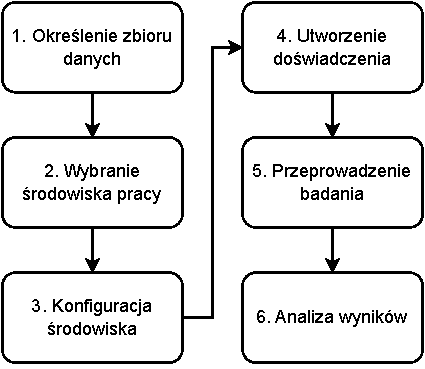
\includegraphics[width=0.9\textwidth]{images/schemat_pracy}
    \captionsource{Schemat przebiegu doświadczenia}{Opracowanie własne}
    \label{fig:sch-prac}
\end{figure}

\vfill
\pagebreak

\section{Założenie techniczne}

Dane prezentowane w \refsource{Tabeli}{tab:technical} określają podstawowe założenia techniczne przyjęte w trakcie wykonywania analizy porównawczej.\ Dane te dotyczą między innymi środowiska, w którym wykonane było doświadczenie.\ Dodatkowo uwzględniono zestaw danych oraz biblioteki użyte w trakcie tworzenia doświadczenia.

\begin{table}[H]
    \centering
    \captionsource{Założenia techniczne pracy dyplomowej}{Opracowanie własne}
    \label{tab:technical}
    \begin{tabular}{|l|l|}
        \hline
        \textbf{Środowisko uruchomieniowe} & Machine Learning Studio\cite{azureml} \\ \hline
        \textbf{Język programowania} & Python 3.x \\ \hline
        \multirow{3}*{\textbf{Wykorzystane biblioteki}} & scikit-learn~\cite{scikit-learn} \\
        \cline{2-2}
        & Numpy~\cite{Harris2019} \\
        \cline{2-2}
        & Pandas~\cite{pandas, McKinney2010} \\
        \hline
        \textbf{Wykorzystane dane} & CICDS2017~\cite{cicds2017kaggle} \\
        \hline
    \end{tabular}
\end{table}

\section{Dane}
\label{sec:data}
Zbiór danych został przygotowany przez Kanadyjski Instytut Cyberbezpieczeństwa działający przy Uniwersytecie Nowy Brunszwik.\ Został wykonany za pomocą narzędzia CICFlowMeter
~\cite{Ahlashkari2022}.\ Zbiór zawiera 79 cech ruchu sieciowego, do których zaliczyć można:
\begin{enumerate}
    \item etykietę,
    \item czas trwania przesyłu,
    \item minimalną długość pakietu zwrotnego,
    \item maksymalną długość pakietu zwrotnego,
    \item port docelowy,
    \item długość pakietów.
\end{enumerate}
Zbiór pozwala na określenie czy ruch sieciowy jest życzliwy \trans{ang. BENING}, czy nieżyczliwy (różne możliwe formy ataku na sieć).\ Dodatkowo zbiór został podzielony na pięć dni roboczych: poniedziałek 3.07.2017 - piątek 7.07.2017.\ Dane z poniedziałku zawierają jedynie ruch życzliwy.\ W pozostałe dni zostały zasymulowane ataki na sieć komputerową~\cite{Blyszcz2022, unbkaggle}.

\section{Programistyczne środowisko badawcze}
Jako środowisko programistyczne zostało wybrane Azure Machine Learning Studio.\ Zostało to spowodowane możliwością uniezależnienia obliczeń od komputera lokalnego.\ Platforma umożliwia łatwy sposób na tworzenie skomplikowanych potoków zadań, które składają się z komponentów wielokrotnego użytku.\ Każdy komponent uruchamia się w środowisku odizolowanym od pozostałych operacji.\ Dzieje się tak dzięki wykorzystaniu wielowęzłowych klastrów obliczeniowych, bazujących na oprogramowaniu Docker.\ Klastry te mogą skalować się w zależności od potrzeb oraz dostępnej jednostki~\cite{MicrosoftLearn2023}.
\\ \\
Całe doświadczenie zostało odwzorowane w graficznym potoku narzędzia ,,\textit{Projektant}'' oraz przedstawione na \refsource{zdjęciu}{fig:pipeline}.

\begin{landscape}
    \centering
\begin{figure}[H]
    \centering
    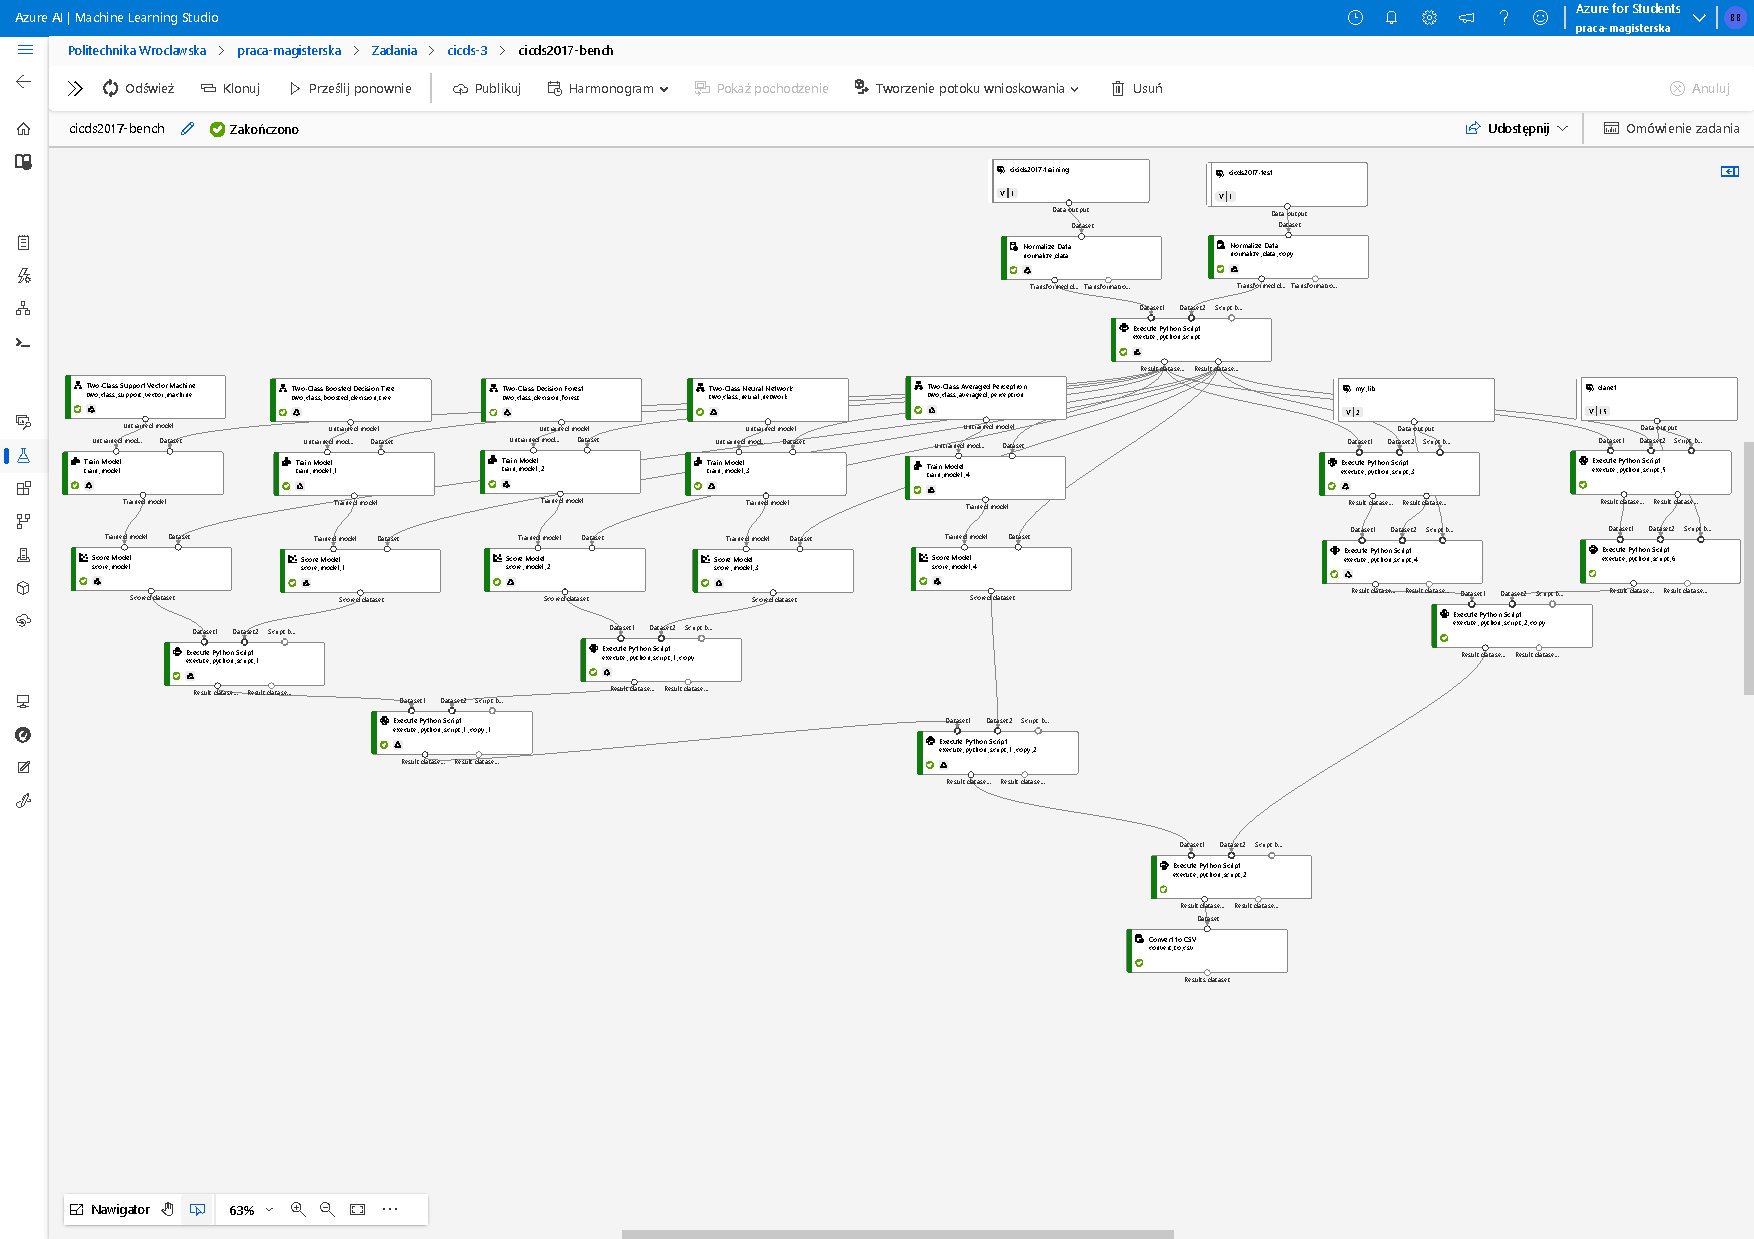
\includegraphics[height=0.9\textwidth]{images/pipeline}
    \captionsource{Potok zadań}{Opracowanie własne}
    \label{fig:pipeline}
\end{figure}
\end{landscape}

\section{Algorytmy}
\label{sec:alg}
W trakcie eksperymenty zastosowano różne algorytmy klasyfikacji danych.\ Charakterystyczną cechą tych algorytmów jest klasyfikacja ukierunkowana na 2 kategorie wejściowe.\ W tym wypadku są to kategorie ruchu sieciowego: [\textbf{BENIGN} \trans{pl. życzliwy}, \textbf{OTHER} \trans{pl. inne}], gdzie inne to pozostałe typy ruchu sieciowego.

\subsection{Two-Class Support Vector Machine}
Algorytm SVM ma za zadanie znaleźć hiperpłaszczyznę w przestrzeni K-wymiarowej (K - liczba cech), która rozdziela zbiory punktów odpowiadających różnym klasom.\ W pierwszej kolejności szuka się separatora między klasami, a następnie przekształca się dane w taki sposób, by można przekształcić separator w hiperpłaszczyznę~\cite{IBM}.\ Sposób działania został zobrazowany za pomocą \refsource{wykresów}{fig:svm-schem}.\ Część \refsource{potoku}{fig:pipeline} odpowiedzialnego za SVM to \refsource{schemat}{fig:svm-pipe}.

\begin{figure}[H]
    \begin{subfigure}[m]{0.45\textwidth}
        \centering
        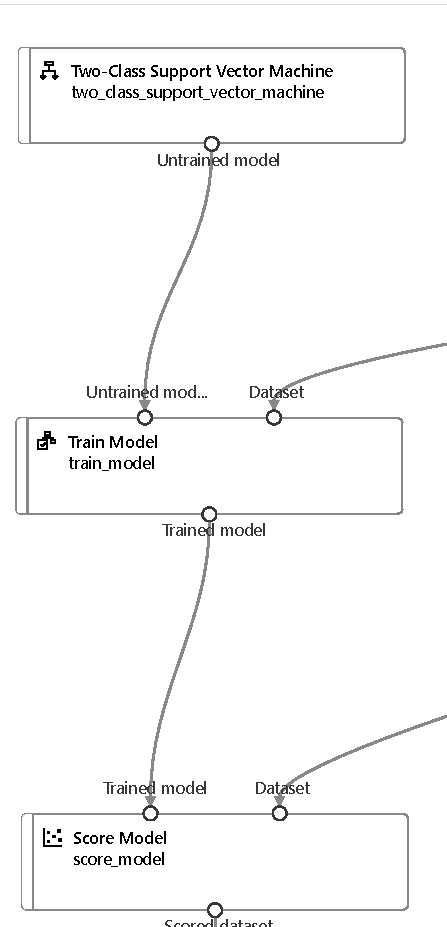
\includegraphics[width=\textwidth]{images/svm_pipe}
        \captionsource{Potok zadań dla modelu \textit{Two-Class Support Vector Machine}}{Opracowanie własne}
        \label{fig:svm-pipe}
    \end{subfigure}
    \hfill
    \begin{subfigure}[m]{0.45\textwidth}
        \centering
        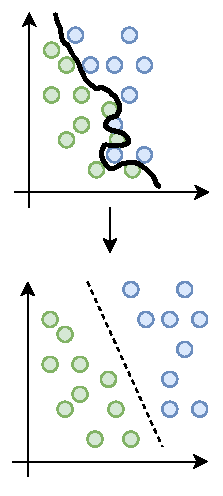
\includegraphics[width=\textwidth]{images/svm}
        \captionsource{Schemat SVM}{\cite{Statsoft}}
        \label{fig:svm-schem}
    \end{subfigure}
\end{figure}

\vfill
\pagebreak

\subsection{Two-Class Boosted Decision Tree}
Jest to algorytm drzewa decyzyjnego oparty o algorytm LightGBM.\ Dzięki zastosowaniu tego podejścia algorytm oparty o drzewo decyzyjne działa szybciej oraz ma mniejszą złożoność obliczeniową.\ Algorytm ten działa na zasadzie doboru odpowiedniego liścia, zamiast jak w przypadku klasycznych algorytmów opartych na drzewie, wyboru odpowiedniej warstwy~\cite{LightGBM}.\ Sposób podejścia liściastego został ukazany na \refsource{schemacie}{fig:leaf}.\ Model wykorzystywany w Azure ML został ukazany na \refsource{rysunku}{fig:dt-pipe}.
\begin{figure}[H]
    \begin{subfigure}[m]{0.3\textwidth}
        \centering
        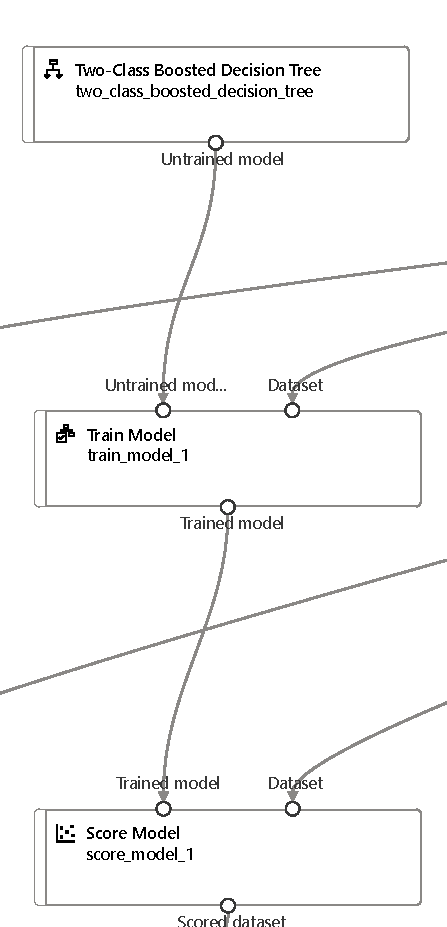
\includegraphics[width=\textwidth]{images/dt_pipe}
        \captionsource{Potok zadań dla modelu \textit{Two-Class Boosted Decision Tree}}{Opracowanie własne}
        \label{fig:dt-pipe}
    \end{subfigure}
    \hfill
    \begin{subfigure}[m]{0.66\textwidth}
        \begin{subfigure}[m]{\textwidth}
            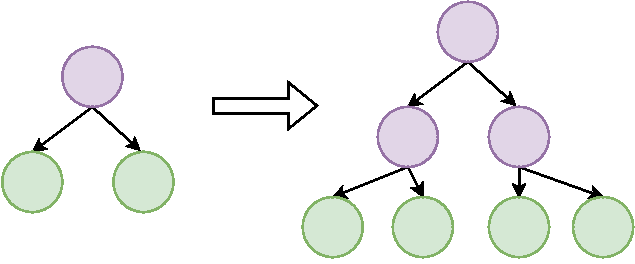
\includegraphics[width=\textwidth]{images/level-wise}
        \end{subfigure}
        \begin{subfigure}[m]{\textwidth}
            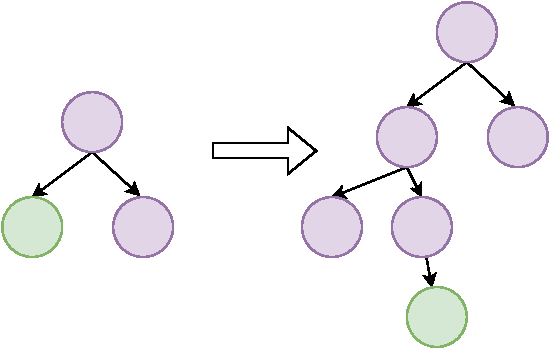
\includegraphics[width=\textwidth]{images/leaf-wise}
        \end{subfigure}
        \captionsource{Sposób działania algorytmu}{\cite{LightGBM}}
        \label{fig:leaf}
    \end{subfigure}
\end{figure}
\vfill
\pagebreak

\subsection{Two-Class Decision Forest}
Las decyzyjny to algorytm, którego wynik opiera się o agregację wyników wielu drzew decyzyjnych.\ Uzyskanie wyniku zależy od algorytmu trenowania lasu.\ Przykładowo w klasyfikacji losowym lasem wieloklasowym \trans{ang. Multi-class random forest classification}, każde drzewo głosuje na jedną klasę.\ Klasa, która zostanie wybrana większością głosów, zostaje uznana za wynikową~\cite{Google}.\ Model wykorzystany w Azure ML pokazano na \refsource{modelu}{fig:df-pipe}

\begin{figure}[H]
    \centering
    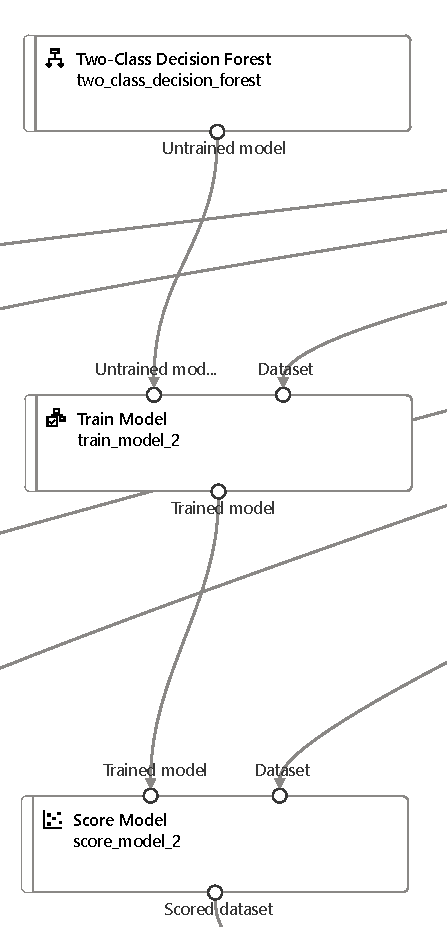
\includegraphics[width=0.3\textwidth]{images/df_pipe}
    \captionsource{Potok zadań dla modelu \textit{Two-Class Decision Forest}}{Opracowanie własne}
    \label{fig:df-pipe}
\end{figure}

\vfill
\pagebreak

\subsection{Two-class Neural Network}
Jest to sieć neuronowa, która składa się z warstwy wejściowej, trzech warstw ukrytych (każda posiada po 100 węzłów), oraz z warstwy wyjściowej.\ Przykładowa sieć neuronowa została zobrazowana na \refsource{schemacie}{fig:neural-network}.\ Moduł wykorzystany w Azure ML ukazano na \refsource{rysunku}{fig:nn-pipe}.

\begin{figure}[H]
    \centering
    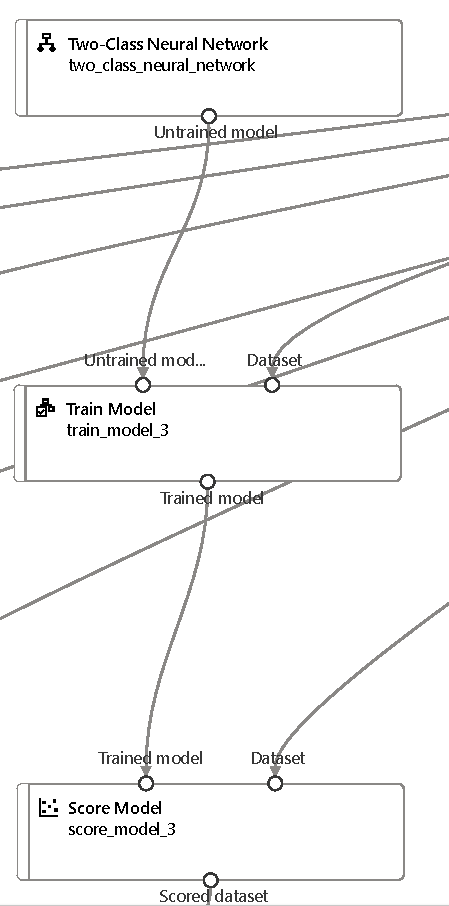
\includegraphics[width=0.3\textwidth]{images/nn_pipe}
    \captionsource{Potok zadań dla modelu \textit{Two-Class Neural Network}}{Opracowanie własne}
    \label{fig:nn-pipe}
\end{figure}

\vfill
\pagebreak

\subsection{Two-Class Average Perceptron}
Jest to najprostsza odmiana sieci neuronowej, czyli pojedynczy perceptron, który jest matematycznym modelem neuronu.\ Składa się on z \textit{n} wejść, takiej samej ilości wag, progu $\Theta$, sumatora, funkcji aktywującej i wyjścia.\ Został zobrazowany na \refsource{schemacie}{fig:neuron}.\ Może służyć za prosty klasyfikator binarny albo za regresor.\ Model wykorzystany w Azure ML ukazano na \refsource{zdjęciu}{fig:ap-pipe}.

\begin{figure}[H]
    \centering
    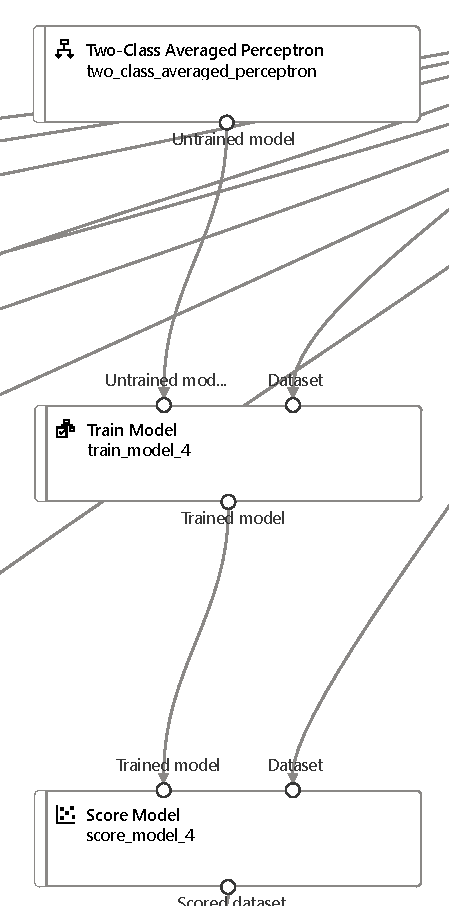
\includegraphics[width=0.3\textwidth]{images/ap_pipe}
    \captionsource{Potok zadań dla modelu \textit{Two-Class Average Perceptron}}{Opracowanie własne}
    \label{fig:ap-pipe}
\end{figure}

\vfill
\pagebreak

\subsection{Gausian Naive Bayes - with GA}
Algorytm ten polega na połączeniu algorytmu genetycznego (GA) wraz z klasyfikatorem naiwnym Bayesa wykorzystującego rozkład Gaussa (GNB).\ Zadaniem algorytmu genetycznego jest znalezienie najistotniejszych cech w zbiorze tabelarycznym.\ Poszukiwane cechy powinny pozwolić na zmniejszenie wymiarowości danych oraz na zmniejszenie kosztów obsługi samego klasyfikatora.\ Co może zostać uzyskane późniejszych etapach testowania, ze względu na zmniejszoną ilość danych wymaganych do przetworzenia.\ GA wykorzystywał w metodzie \textbf{fitness} algorytm GNB w celu określenia dopasowania danych.\ Zadaniem GNB było znalezienie najlepszej dostępnej kombinacji cech, które pozwalały na uzyskanie najlepszego dopasowania~\cite{Blyszcz2022}.\ Model wykorzystywany w Azure ML różni się od gotowych modeli tym, że dołączono do niego bibliotekę napisaną w języku Python, która zawiera kod wykorzystywany w pracy inżynierskiej autora~\cite{Suvres2023}.
\begin{figure}[H]
    \centering
    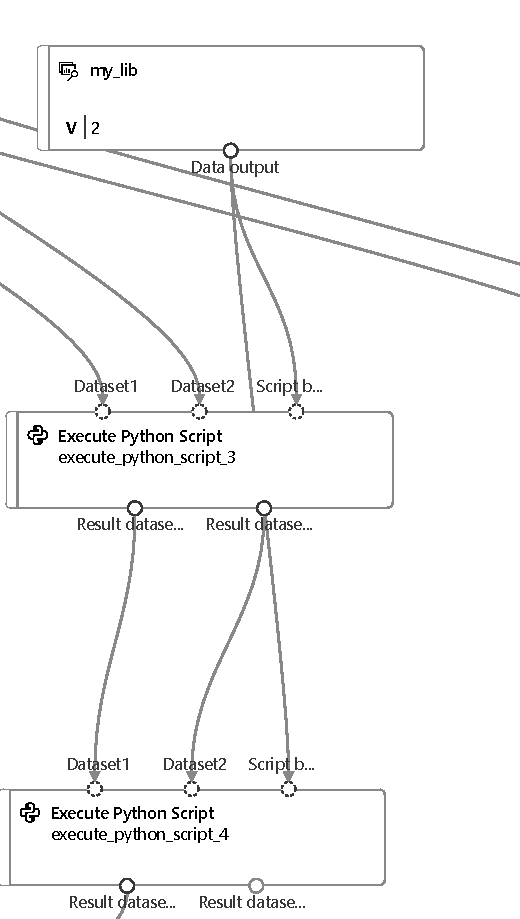
\includegraphics[width=0.3\textwidth]{images/ga_pipe}
    \captionsource{Potok zadań dla modelu}{Opracowanie własne}
    \label{fig:ga-pipe}
\end{figure}

\vfill
\pagebreak

\subsection{DANet}
Twórcy tego algorytmu wprowadzają dodatkową warstwę abstrakcyjną o nazwie ,,\textit{Abstract Layer}''.\ Warstwy te budują sieć o nazwie ,,\textit{Deep Abstract Network}'' (DANet).\ Zadanie dodatkowych warstw jest grupowanie cech w skorelowanych zbiorach.\ Zbiory te budują sieć powiązań między sobą w formie sieci semantycznej.\ Gdy sieć semantyczna jest zbudowana, to w ostatnim kroku wykonywana jest klasyfikacja w trzywarstwowej sieci perceptronów \trans{ang. Multilayer Perceptron network} (MLP)~\cite{Chen2022, Danet}.\ Model znajdujący się z Azure ML został przedstawiony na \refsource{zdjęciu}{fig:danet-pipe}, zaś sposób działania ukazano na \refsource{schematach}{fig:danet-abst}.

\begin{figure}[H]
    \begin{subfigure}[m]{0.49\textwidth}
        \centering
        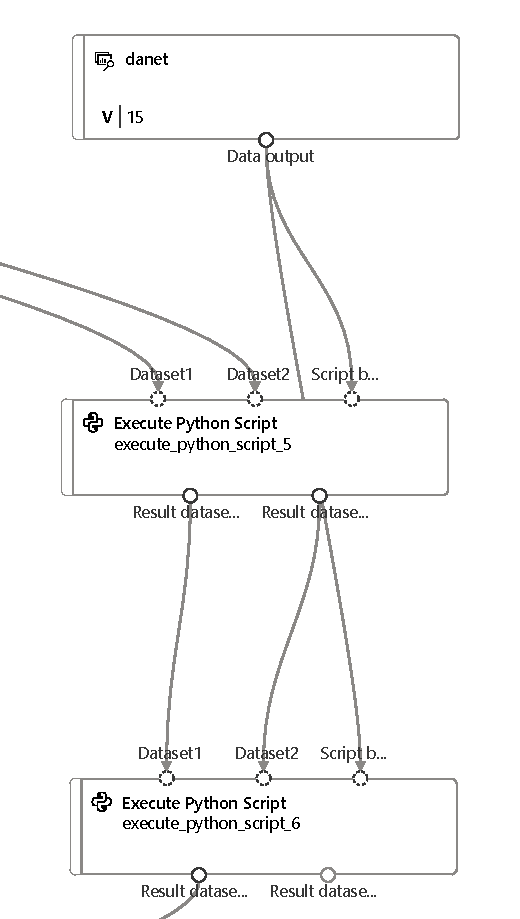
\includegraphics[width=0.4\textwidth]{images/danet}
        \captionsource{Potok zadań dla modelu \textit{DANet}}{Opracowanie własne}
        \label{fig:danet-pipe}
    \end{subfigure}
    \hfill
    \begin{subfigure}[m]{0.49\textwidth}
        \begin{subfigure}[m]{\textwidth}
            \centering
            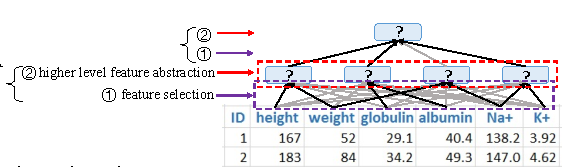
\includegraphics[width=\textwidth]{images/danet_1}
        \end{subfigure}
        \begin{subfigure}[m]{\textwidth}
            \centering
            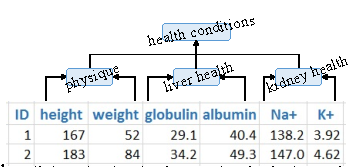
\includegraphics[width=\textwidth]{images/danet_2}
        \end{subfigure}
        \captionsource{Sposób działania DANet}{\cite{Chen2022}}
        \label{fig:danet-abst}
    \end{subfigure}

\end{figure}





\chapter{Podsumowanie}
Niniejsza praca magisterska miała na celu, wykonanie porównania algorytmów klasyfikacyjnych dostarczonych przez platformę Azure, wraz z GAGNB oraz algorytmem DANet.\ Wśród autorskich algorytmów znajdywał się algorytm opracowany przez autora pracy magisterskiej - \textit{Gaussian Naive Bayes - with GA}.\ Miało to na celu sprawdzenie, czy tworzenie autorskich rozwiązań nakierowanych na problem będzie opłacalne w dobie gotowych rozwiązań.
\\ \\
W pracy dokonano przeglądu literaturowego związanego zagadnieniem uczenia maszynowego oraz z podejściem low-code/no-code.\ Dzięki temu wybrano narzędzie Machine Learning Studio znajdujące się na platformie Microsoft Azure. \ Microsoft wyszedł naprzeciw potrzebom użytkowników, przygotowując zestaw prekonfigurowanych algorytmów klasyfikacyjnych.\ Możliwości narzędzia Azure ML pozwalają na tworzenie wysokoskalowalnych rozwiązań z zakresu uczenia maszynowego przy relatywnie niskich kosztach.\ Jednakże mogą wystąpić specyficzne wymagania biznesowe albo prawne, które nie będą pozwalały na zastosowanie zewnętrznych narzędzi chmurowych.\ Takim przykładem są strategiczne dane państwowe, których wyciek za granicą może grozić poważnym zagrożeniem z zewnątrz.\ W przypadku systemów wykrywania intruzów zasadne jest stosowanie autorskich rozwiązań, które nie są znane opinii publicznej.\ Takie działanie chroni przed nieautoryzowanym dostępem do sieci komputerowej oraz do danych wrażliwych.
\\ \\
Konkurencyjność rozwiązań autorskich przedstawiono na \refsource{wykresie}{fig:predict-result}.\ Wykorzystanie połączenia algorytmu genetycznego i klasyfikatora naiwnego Bayesa z rozkładem normalnym pozwala na uzyskanie zbliżonych wyników do algorytmu utworzonych przez Microsoft.\ Różnica około 5 punktów procentowych między najlepszym algorytmem a algorytmem \textit{Gaussian Naive Bayes - with GA} ukazuje niewielką różnicę w jakości algorytmu.\ Częstą wadą autorskich rozwiązań jest ich nakierowanie na konkretny zestaw danych.\ Zostało to pokazane podczas wykorzystania algorytmu DANet, który dobrze sklasyfikował dane związane z m.in. chorobami serca~\cite{Chen2022}.\ Algorytm ten jednakże błędnie skategoryzował dane związane z ruchem sieciowym.
\\ \\
Dodatkowo korzystanie z tego typu prostych rozwiązań autorskich pozwala na prototypownie rozwiązań biznesowych opartych o klasyfikację danych.\ Zastosowanie algorytmu \textit{GAGNB} nie wymaga wcześniejszej znajomości zbioru danych.\ Pozwala na lokalne korzystanie z programu do klasyfikacji, bez ponoszenia kosztów wykorzystania platformy chmurowej.\ Kolejnym atutem tego algorytmu jest zmniejszenie kosztów lokalnego użytkowania.\ Co zostało spowodowane zmniejszeniem wymiarowości zbioru danych do klasyfikacji poprzez wykorzystanie jedynie wytypowanych kolumn.
\\ \\
Stworzony projekt jest jedynie silnikiem klasyfikacyjnym, który pozwala na wytrenowanie i wyłonienie najlepszego algorytmu do klasyfikacji danych.\ Dzięki możliwościom platformy Azure ML stworzenie całego środowiska testowego jest relatywnie tanie i nie wymaga wielu wyspecjalizowanych umiejętności.\ Bazując na wynikach i najlepszym klasyfikatorze, można utworzyć odpowiednie przepływy służące do klasyfikacji danych wejściowych.\ Dostęp do nich może odbywać się za pomocą utworzonych Punktów Dostępowych \trans{ang. Endpoints}.\ Dzięki punktom dostępowym możliwa jest komunikacja za pomocą protokołu HTTPS \trans{ang. Hyper Text Transfer Protocol Secure} i komunikacja typu REST \textit{(ang. Representative State Transfer)}.
\\ \\
Utworzony w ten sposób punkt dostępu może zostać wykorzystany w klasyfikacji ruchu sieciowego w niewielkich aplikacjach z dostępem do internetu.\ Pozwoliłoby to na realizację analizy danych w chmurze, co mogłoby przyspieszyć cały proces oraz utworzyć pojedyncze źródło prawdy dla wielu instancji aplikacji.\ A wykorzystanie dodatkowo konteneryzacji, którą zapewnia platforma Azure, cały proces mógłby zostać zoptymalizowany pod kątem wydajnościowym i lokalizacyjnym.\ Pojedyncze źródło prawdy jest zaletą wykorzystania ,,\textit{zewnętrznego}'' klasyfikatora, ponieważ zapewnia jednakowe wyniki klasyfikacji w poszczególnych instancjach samej aplikacji instalowanej na wielu urządzeniach.\ Pozwala to również na lepsze dostrajanie całego procesu, a wykorzystanie kolejnych wersji przepływów umożliwia utrzymywanie kopii zapasowych poszczególnych rozwiązań.\ Umożliwia to na przykład cofnięcie wersji klasyfikatora w przypadku wykrycia nieprawidłowości w obecnym modelu.


% LITERATURA (zostanie wygenerowana automatycznie)
%UWAGA: bibliotekę referencji należy przygotować samemu. Dobrym do tego narzędziem jest JabRef.
%       JabRef oferuje jednak większą liczbę typów rekordów niż obsługuje BibTeX.
%       Proszę nie deklarować rekordów o typach nieobsługiwanych przez BibTeX.
%       Formatowania wykazu literatury i cytowań odbywać się ma zgodnie z zadeklarowanym stylem.
%       Zalecane są style produkujące numeryczne cytowania (w postaci [1], [2,3]).
%       Takim stylem jest np. plabbrv
%\bibliographystyle{plabbrv}
%       Aby zapanować nad odstępami w wykazie literatury można posłużyć się poniższą komendą
%\setlength{\bibitemsep}{2pt} % - zacieśnia wykaz
%       Pozycja Literatura pojawia się w spisie treści nieco inaczej niż spisy rysunków, tabel itp.
%       Aby zachować właściwe odstępy należy użyć poniższej komendy
%       Nazwę pliku przygotowanej biblioteki wpisuje się bez rozszerzenia .bib
%       (linia poniżej załaduje rekordy z pliku "dokumentacja.bib")
%\bibliography{dokumentacja}


\printbibliography[title={Literatura}]


% Nie wyświetlaj wybranych pól.
%\AtEveryBibitem{\clearfield{note}}


%\appendix
% \include{dodatekA}
% \include{dodatekB}

% Jeśli w pracy pojawiać się ma indeks, należy odkomentować poniższe linie
%%\chapterstyle{noNumbered}
%%\phantomsection % sets an anchor
%%\addcontentsline{toc}{chapter}{Indeks rzeczowy}
%%\printindex

\end{document}
